\documentclass[]{book}
\usepackage{lmodern}
\usepackage{amssymb,amsmath}
\usepackage{ifxetex,ifluatex}
\usepackage{fixltx2e} % provides \textsubscript
\ifnum 0\ifxetex 1\fi\ifluatex 1\fi=0 % if pdftex
  \usepackage[T1]{fontenc}
  \usepackage[utf8]{inputenc}
\else % if luatex or xelatex
  \ifxetex
    \usepackage{mathspec}
  \else
    \usepackage{fontspec}
  \fi
  \defaultfontfeatures{Ligatures=TeX,Scale=MatchLowercase}
\fi
% use upquote if available, for straight quotes in verbatim environments
\IfFileExists{upquote.sty}{\usepackage{upquote}}{}
% use microtype if available
\IfFileExists{microtype.sty}{%
\usepackage{microtype}
\UseMicrotypeSet[protrusion]{basicmath} % disable protrusion for tt fonts
}{}
\usepackage{hyperref}
\hypersetup{unicode=true,
            pdftitle={Data Programming 數據編程學},
            pdfauthor={Karl Ho 何嘉耀 (洪碩廷 翻譯)},
            pdfborder={0 0 0},
            breaklinks=true}
\urlstyle{same}  % don't use monospace font for urls
\usepackage{natbib}
\bibliographystyle{apalike}
\usepackage{color}
\usepackage{fancyvrb}
\newcommand{\VerbBar}{|}
\newcommand{\VERB}{\Verb[commandchars=\\\{\}]}
\DefineVerbatimEnvironment{Highlighting}{Verbatim}{commandchars=\\\{\}}
% Add ',fontsize=\small' for more characters per line
\usepackage{framed}
\definecolor{shadecolor}{RGB}{248,248,248}
\newenvironment{Shaded}{\begin{snugshade}}{\end{snugshade}}
\newcommand{\AlertTok}[1]{\textcolor[rgb]{0.94,0.16,0.16}{#1}}
\newcommand{\AnnotationTok}[1]{\textcolor[rgb]{0.56,0.35,0.01}{\textbf{\textit{#1}}}}
\newcommand{\AttributeTok}[1]{\textcolor[rgb]{0.77,0.63,0.00}{#1}}
\newcommand{\BaseNTok}[1]{\textcolor[rgb]{0.00,0.00,0.81}{#1}}
\newcommand{\BuiltInTok}[1]{#1}
\newcommand{\CharTok}[1]{\textcolor[rgb]{0.31,0.60,0.02}{#1}}
\newcommand{\CommentTok}[1]{\textcolor[rgb]{0.56,0.35,0.01}{\textit{#1}}}
\newcommand{\CommentVarTok}[1]{\textcolor[rgb]{0.56,0.35,0.01}{\textbf{\textit{#1}}}}
\newcommand{\ConstantTok}[1]{\textcolor[rgb]{0.00,0.00,0.00}{#1}}
\newcommand{\ControlFlowTok}[1]{\textcolor[rgb]{0.13,0.29,0.53}{\textbf{#1}}}
\newcommand{\DataTypeTok}[1]{\textcolor[rgb]{0.13,0.29,0.53}{#1}}
\newcommand{\DecValTok}[1]{\textcolor[rgb]{0.00,0.00,0.81}{#1}}
\newcommand{\DocumentationTok}[1]{\textcolor[rgb]{0.56,0.35,0.01}{\textbf{\textit{#1}}}}
\newcommand{\ErrorTok}[1]{\textcolor[rgb]{0.64,0.00,0.00}{\textbf{#1}}}
\newcommand{\ExtensionTok}[1]{#1}
\newcommand{\FloatTok}[1]{\textcolor[rgb]{0.00,0.00,0.81}{#1}}
\newcommand{\FunctionTok}[1]{\textcolor[rgb]{0.00,0.00,0.00}{#1}}
\newcommand{\ImportTok}[1]{#1}
\newcommand{\InformationTok}[1]{\textcolor[rgb]{0.56,0.35,0.01}{\textbf{\textit{#1}}}}
\newcommand{\KeywordTok}[1]{\textcolor[rgb]{0.13,0.29,0.53}{\textbf{#1}}}
\newcommand{\NormalTok}[1]{#1}
\newcommand{\OperatorTok}[1]{\textcolor[rgb]{0.81,0.36,0.00}{\textbf{#1}}}
\newcommand{\OtherTok}[1]{\textcolor[rgb]{0.56,0.35,0.01}{#1}}
\newcommand{\PreprocessorTok}[1]{\textcolor[rgb]{0.56,0.35,0.01}{\textit{#1}}}
\newcommand{\RegionMarkerTok}[1]{#1}
\newcommand{\SpecialCharTok}[1]{\textcolor[rgb]{0.00,0.00,0.00}{#1}}
\newcommand{\SpecialStringTok}[1]{\textcolor[rgb]{0.31,0.60,0.02}{#1}}
\newcommand{\StringTok}[1]{\textcolor[rgb]{0.31,0.60,0.02}{#1}}
\newcommand{\VariableTok}[1]{\textcolor[rgb]{0.00,0.00,0.00}{#1}}
\newcommand{\VerbatimStringTok}[1]{\textcolor[rgb]{0.31,0.60,0.02}{#1}}
\newcommand{\WarningTok}[1]{\textcolor[rgb]{0.56,0.35,0.01}{\textbf{\textit{#1}}}}
\usepackage{longtable,booktabs}
\usepackage{graphicx,grffile}
\makeatletter
\def\maxwidth{\ifdim\Gin@nat@width>\linewidth\linewidth\else\Gin@nat@width\fi}
\def\maxheight{\ifdim\Gin@nat@height>\textheight\textheight\else\Gin@nat@height\fi}
\makeatother
% Scale images if necessary, so that they will not overflow the page
% margins by default, and it is still possible to overwrite the defaults
% using explicit options in \includegraphics[width, height, ...]{}
\setkeys{Gin}{width=\maxwidth,height=\maxheight,keepaspectratio}
\IfFileExists{parskip.sty}{%
\usepackage{parskip}
}{% else
\setlength{\parindent}{0pt}
\setlength{\parskip}{6pt plus 2pt minus 1pt}
}
\setlength{\emergencystretch}{3em}  % prevent overfull lines
\providecommand{\tightlist}{%
  \setlength{\itemsep}{0pt}\setlength{\parskip}{0pt}}
\setcounter{secnumdepth}{5}
% Redefines (sub)paragraphs to behave more like sections
\ifx\paragraph\undefined\else
\let\oldparagraph\paragraph
\renewcommand{\paragraph}[1]{\oldparagraph{#1}\mbox{}}
\fi
\ifx\subparagraph\undefined\else
\let\oldsubparagraph\subparagraph
\renewcommand{\subparagraph}[1]{\oldsubparagraph{#1}\mbox{}}
\fi

%%% Use protect on footnotes to avoid problems with footnotes in titles
\let\rmarkdownfootnote\footnote%
\def\footnote{\protect\rmarkdownfootnote}

%%% Change title format to be more compact
\usepackage{titling}

% Create subtitle command for use in maketitle
\providecommand{\subtitle}[1]{
  \posttitle{
    \begin{center}\large#1\end{center}
    }
}

\setlength{\droptitle}{-2em}

  \title{Data Programming 數據編程學}
    \pretitle{\vspace{\droptitle}\centering\huge}
  \posttitle{\par}
    \author{Karl Ho 何嘉耀 (洪碩廷 翻譯)}
    \preauthor{\centering\large\emph}
  \postauthor{\par}
      \predate{\centering\large\emph}
  \postdate{\par}
    \date{2019-05-29}

\usepackage{booktabs}
\usepackage{amsthm}
\makeatletter
\def\thm@space@setup{%
  \thm@preskip=8pt plus 2pt minus 4pt
  \thm@postskip=\thm@preskip
}
\makeatother
\usepackage{fontspec}
\setmainfont{Arial}

\begin{document}
\maketitle

{
\setcounter{tocdepth}{1}
\tableofcontents
}
\hypertarget{section}{%
\chapter{課前準備}\label{section}}

本課程不需要任何寫程式經驗。但是,如果您有一些寫程式經驗(例如SPSS,Stata,HTML),它將會有所幫助。R,Python和JavaScript都是直譯語言。換句話說,程序不需要編譯,可以在開發環境中直接執行。
所有套件和帳戶都是免費的,並由開源提供支持。建議學生攜帶自己的筆記型電腦(不是移動裝置)運行MacOS,Linux或Windows操作系統。

推薦的軟體和編譯器:

\begin{enumerate}
\def\labelenumi{\arabic{enumi}.}
\tightlist
\item
  R(\url{https://cran.r-project.org})
\item
  RStudio(\url{https://www.rstudio.com})
\item
  Anaconda 3(\url{https://www.anaconda.com})*
\item
  自己選擇的文本編輯器(例如Atom,Sublime Text,Ultraedit)
\end{enumerate}

推薦的網站/帳戶:

\begin{enumerate}
\def\labelenumi{\arabic{enumi}.}
\tightlist
\item
  GitHub(\url{https://github.com})
\item
  RStudio Cloud
  (*) - 僅限Python 3.x.
\end{enumerate}

\hypertarget{intro}{%
\chapter{簡介}\label{intro}}

本章介紹資料程式設計的一般原則。資料程式設計是一種隨資料一起工作和發展的實踐。與點擊式方法不同,程式設計允許用戶以更有效的方式管理資料和處理資料。程式旨在由用戶和協作者進行複制。可以迭代地和遞增地開發和更新資料程式。換句話說,它是建立不重複的步驟達成高效率的成品。它需要調整測試,這是除錯的過程,但事實上,程式工程師自己在未來的工作中可以使用不同的輸入,或者在使用狀況不同的時候,來更新程式不同的情況。

\hypertarget{section-1}{%
\section{程式設計原則}\label{section-1}}

\href{http://home.bi.no/charlotte.ostergaard/students/CodeAndData.pdf}{社會科學家 Gentzkow and Shapiro (2014)} 列出了資料程式設計的一些原則。

\begin{enumerate}
\def\labelenumi{\arabic{enumi}.}
\tightlist
\item
  自動化
\end{enumerate}

\begin{itemize}
\tightlist
\item
  可複制性(不過時,面向未來)
\end{itemize}

\begin{enumerate}
\def\labelenumi{\arabic{enumi}.}
\setcounter{enumi}{1}
\tightlist
\item
  版本控制
\end{enumerate}

\begin{itemize}
\tightlist
\item
  允許進化和更新版本
\item
  使用Git和GitHub
\end{itemize}

\begin{enumerate}
\def\labelenumi{\arabic{enumi}.}
\setcounter{enumi}{2}
\tightlist
\item
  目錄
\end{enumerate}

\begin{itemize}
\tightlist
\item
  按功能組織
\end{itemize}

\begin{enumerate}
\def\labelenumi{\arabic{enumi}.}
\setcounter{enumi}{3}
\tightlist
\item
  索引
\end{enumerate}

\begin{itemize}
\tightlist
\item
  索引變數(關係型數據庫)
\end{itemize}

\begin{enumerate}
\def\labelenumi{\arabic{enumi}.}
\setcounter{enumi}{4}
\tightlist
\item
  簡約化
\end{enumerate}

\begin{itemize}
\tightlist
\item
  KISS(保持簡短)
\end{itemize}

\begin{enumerate}
\def\labelenumi{\arabic{enumi}.}
\setcounter{enumi}{5}
\tightlist
\item
  紀錄
\end{enumerate}

\begin{itemize}
\tightlist
\item
  給後續使用者的註解
\end{itemize}

\begin{enumerate}
\def\labelenumi{\arabic{enumi}.}
\setcounter{enumi}{6}
\tightlist
\item
  管理
\end{enumerate}

\begin{itemize}
\tightlist
\item
  準備作共同開發
\end{itemize}

\hypertarget{section-2}{%
\section{資料程式的功能}\label{section-2}}

一個數據程式可以具備或執行以下功能:
1. 紀錄數據內容
2. 導入和導出數據
3. 管理數據
4. 數據視覺化
5. 數據模型

Sample R Programs R 程式範例:

\emph{R basics 基本程式}

\begin{Shaded}
\begin{Highlighting}[]
\CommentTok{# Create variables composed of random numbers}
\NormalTok{x <-}\KeywordTok{rnorm}\NormalTok{(}\DecValTok{50}\NormalTok{) }
\NormalTok{y =}\StringTok{ }\KeywordTok{rnorm}\NormalTok{(x)}

\CommentTok{# Plot the points in the plane 平面制圖 }
\KeywordTok{plot}\NormalTok{(x, y)}
\end{Highlighting}
\end{Shaded}

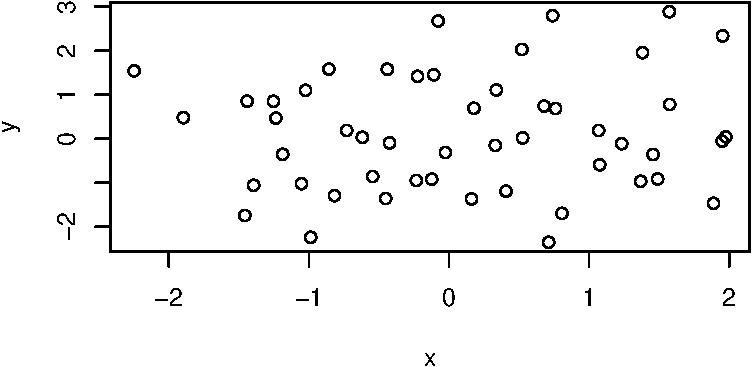
\includegraphics{DataProgramming_files/figure-latex/unnamed-chunk-1-1.pdf}

\emph{Using R packages R 組件包}

\begin{Shaded}
\begin{Highlighting}[]
\CommentTok{# Plot better, using the ggplot2 package }
\CommentTok{## Prerequisite: install and load the ggplot2 package}
\CommentTok{## install.packages("ggplot2")}
\KeywordTok{library}\NormalTok{(ggplot2)}
\KeywordTok{qplot}\NormalTok{(x,y)}
\end{Highlighting}
\end{Shaded}

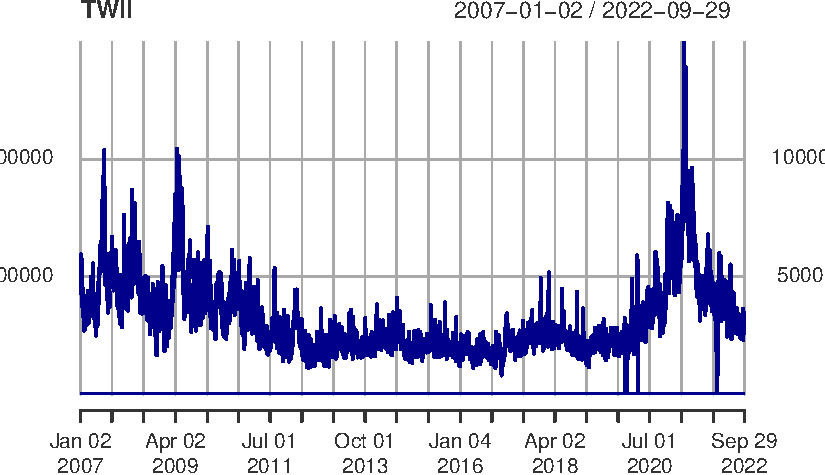
\includegraphics{DataProgramming_files/figure-latex/unnamed-chunk-2-1.pdf}

\emph{More R Data Visualization R 數據視覺化}

\begin{Shaded}
\begin{Highlighting}[]
\CommentTok{# Plot better better with ggplot2}
\KeywordTok{ggplot}\NormalTok{(,}\KeywordTok{aes}\NormalTok{(x,y)) }\OperatorTok{+}\StringTok{ }\KeywordTok{theme_bw}\NormalTok{() }\OperatorTok{+}\StringTok{ }\KeywordTok{geom_point}\NormalTok{(}\DataTypeTok{col=}\StringTok{"blue"}\NormalTok{)}
\end{Highlighting}
\end{Shaded}

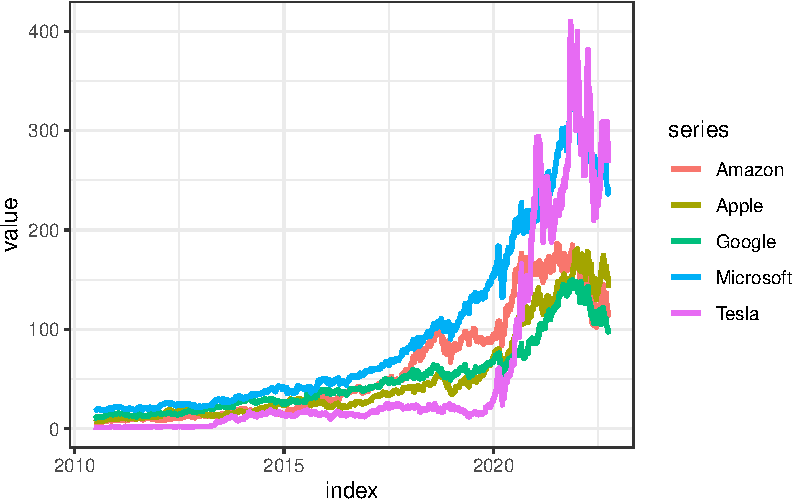
\includegraphics{DataProgramming_files/figure-latex/unnamed-chunk-3-1.pdf}

Sample Python Programs Python 程式範例 (\#\# 代表程式輸出)

\emph{Python using Pandas}

\begin{Shaded}
\begin{Highlighting}[]

\CommentTok{# Import a text file in csv format}
\ImportTok{import}\NormalTok{ pandas }\ImportTok{as}\NormalTok{ pd}
\NormalTok{CO2 }\OperatorTok{=}\NormalTok{ pd.read_csv(}\StringTok{"https://raw.githubusercontent.com/kho777/data-visualization/master/data/CO2.csv"}\NormalTok{)}

\CommentTok{# Take a glimpse of the data file}
\NormalTok{CO2.head()}
\end{Highlighting}
\end{Shaded}

\begin{verbatim}
##                country               CO2 _kt  CO2pc  CO2percent
## 0                       Australia    446,348   18.6       1.23%
## 1                   United States  5,172,336   16.1      14.26%
## 2                    Saudi Arabia    505,565   16.0       1.39%
## 3                          Canada    555,401   15.5       1.53%
## 4                          Russia  1,760,895   12.3       4.86%
\end{verbatim}

\emph{Python using Matplotlib}

\begin{Shaded}
\begin{Highlighting}[]
\CommentTok{# Using matplotlib to do a simple plot}
\ImportTok{import}\NormalTok{ matplotlib.pyplot }\ImportTok{as}\NormalTok{ plt}
\NormalTok{CO2pc}\OperatorTok{=}\NormalTok{CO2[}\StringTok{"CO2pc"}\NormalTok{]}
\NormalTok{plt.plot(CO2pc)}
\end{Highlighting}
\end{Shaded}

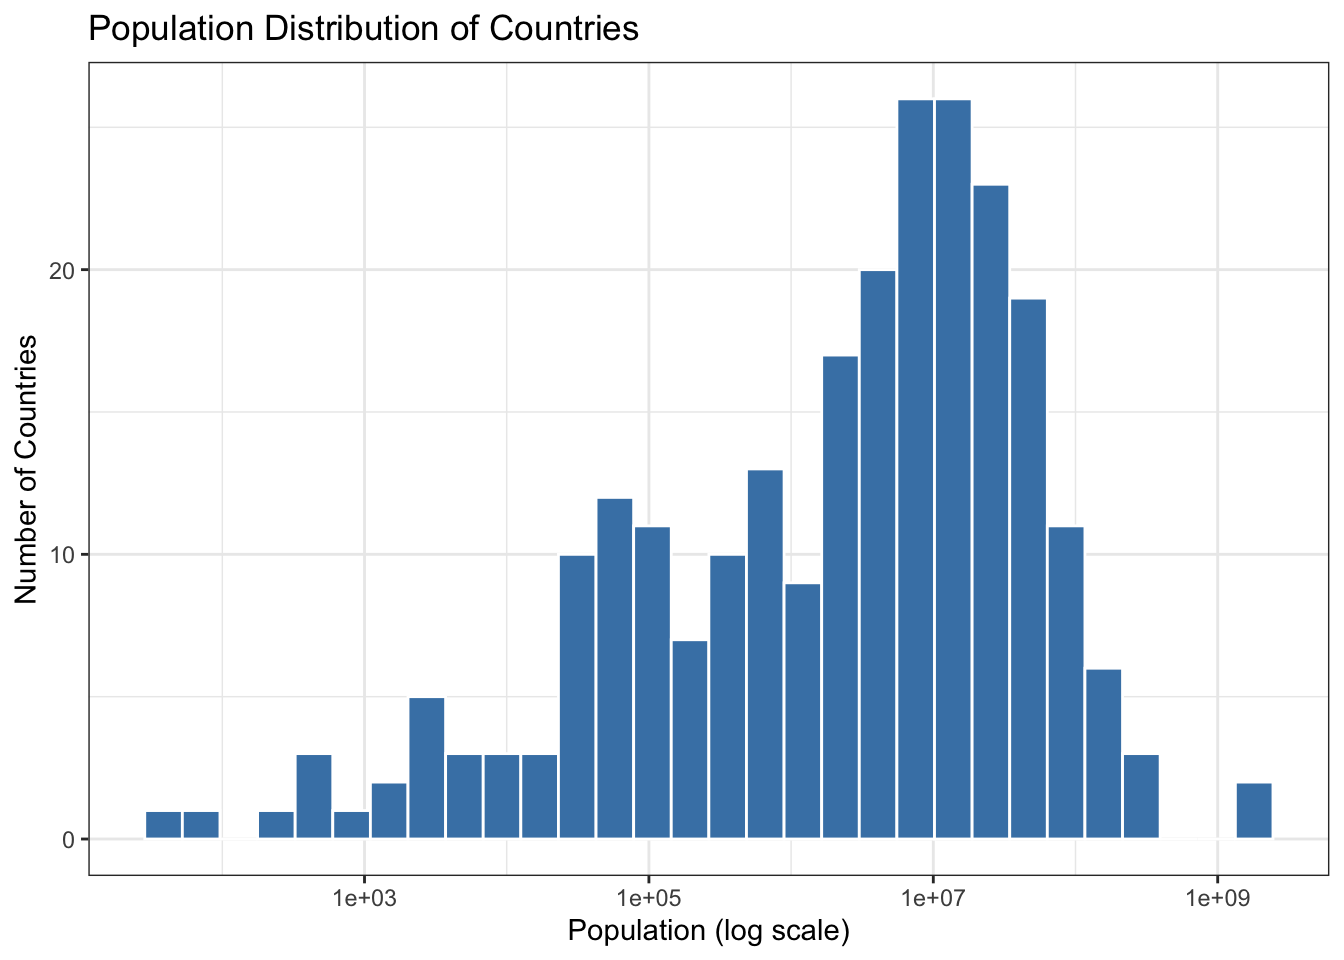
\includegraphics{DataProgramming_files/figure-latex/unnamed-chunk-5-1.pdf}

在接下來的章節中,將提供示範程式來說明這些功能。

\hypertarget{r}{%
\chapter{R語言程式設計}\label{r}}

\hypertarget{r-1}{%
\section{什麼是R?}\label{r-1}}

R統計程式語言是一個免費開源軟件包,以John Chambers開發的S語言作為基礎。

\hypertarget{rs}{%
\subsection{R和S的一些歷史}\label{rs}}

Robert Gentlemen(加拿大)和Ross Ihaka(紐西蘭)將S進一步發展為R。

\begin{figure}
\includegraphics[width=1\linewidth]{Rinventors} \caption{R Inventors}\label{fig:Rinventors}
\end{figure}

Source: \href{https://rss.onlinelibrary.wiley.com/doi/10.1111/j.1740-9713.2018.01169.x}{Nick Thieme. 2018. R Generation: 25 years of R}

\hypertarget{r-2}{%
\subsection{R是:}\label{r-2}}

\begin{itemize}
\tightlist
\item
  很大,可能是最大的基於用戶編寫的附加組件/程式
\item
  物件導向
\item
  互動
\item
  支持多種作業系統:Windows,Mac,Linux
\end{itemize}

根據John Chambers(2009)的解釋,R的六個方面包括:
1. 一個具備多種類運算處理流程的功能介面;
2. 互動,容易上手的;
3. 具備功能性的程式模塊;
4. 物件導向,``一切都是物件'';
5. 模組化,由標準化元件製成;
6. 全世界的開源與協做。

\begin{figure}
\includegraphics[width=1\linewidth]{Rdevelopers} \caption{Prominent R Developers}\label{fig:Rdevelopers}
\end{figure}

Source: \href{https://rss.onlinelibrary.wiley.com/doi/10.1111/j.1740-9713.2018.01169.x}{Nick Thieme. 2018. R Generation: 25 years of R}

\hypertarget{r-3}{%
\section{為何選擇R?}\label{r-3}}

\begin{itemize}
\tightlist
\item
  程式設計平台環境
\item
  允許用戶開發軟體/套件
\item
  目前,CRAN軟件包存儲庫包含超過14,000個可用套件(截至2019年5月)。
\item
  圖像化!
\item
  可擴展和輕便的
\item
  與其他平台/語言的銜接介面(例如C++,Python,JavaScript,Stan,SQL)
\item
  比較R與其他軟件?
\end{itemize}

\begin{figure}
\includegraphics[width=1\linewidth]{Rcompare} \caption{R Compared with other statistical programs/platforms}\label{fig:Rcompare}
\end{figure}

Source: Oscar Torres-Reyna. 2010. \href{https://dss.princeton.edu/training/RStata.pdf}{Getting Started in R\textasciitilde Stata Notes on Exploring Data}

\hypertarget{rstudio}{%
\section{RStudio}\label{rstudio}}

RStudio是統計程式設計軟體R的使用者介面。
- 物件導向的環境
- 視窗化的使用者介面
- 點擊操作
- 編碼推薦
- 擴張和發展
- 多功能整合開發環境(IDE)

\begin{figure}
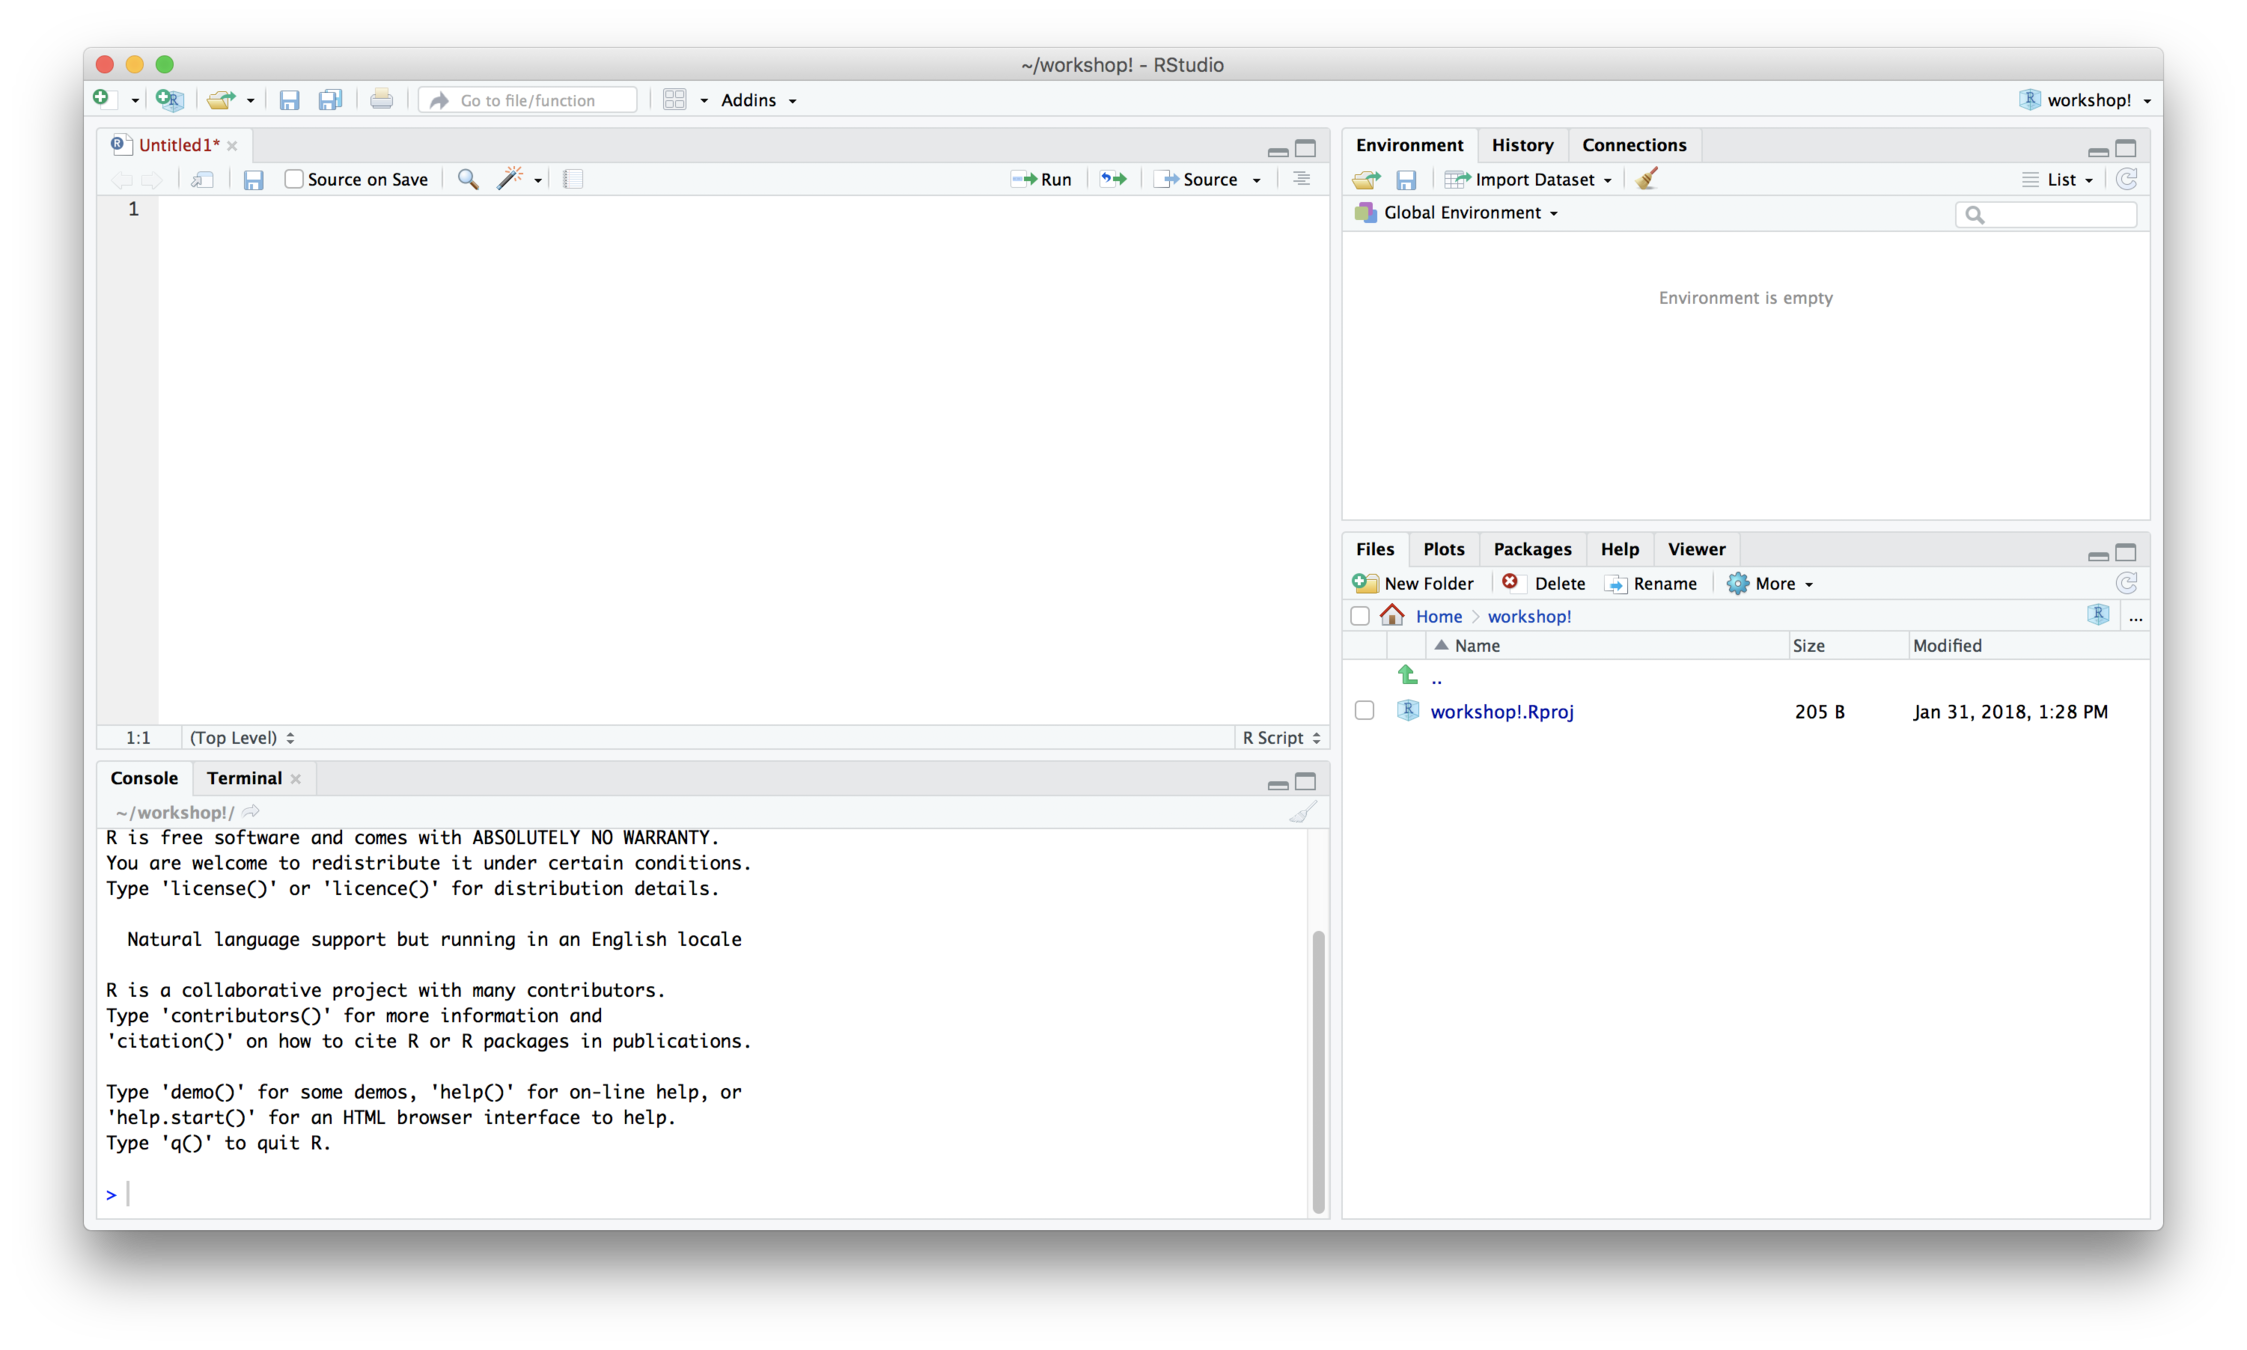
\includegraphics[width=1\linewidth]{RStudioscreenshot} \caption{RStudio screenshot}\label{fig:Rstudioscreenshot}
\end{figure}

\hypertarget{section-3}{%
\section{基本操作和賦值}\label{section-3}}

算術運算:
+, - ,*,/,\^{}是標準算術運算符。
賦值
要為變數賦值,請使用``\textless{} -''或``='':

\begin{Shaded}
\begin{Highlighting}[]
\CommentTok{## Introduction to R sample program }
\CommentTok{## file: introR02.R}
\CommentTok{## Adapted from Venables, W.N., Smith, D.M. and Team, R.C., 2018. An Introduction to R, Version 3.5.1 (2018-07-02)}


\CommentTok{# Clear any existing objects }
\KeywordTok{rm}\NormalTok{(}\DataTypeTok{list =} \KeywordTok{ls}\NormalTok{())}

\CommentTok{# Generate x, y and w to demontrate linear models and plots.}
\CommentTok{# Make x = (1,2,...,20).}

\NormalTok{x <-}\StringTok{ }\DecValTok{1}\OperatorTok{:}\DecValTok{20}

\CommentTok{# Create A ‘weight’ vector of standard deviations.}

\NormalTok{w <-}\StringTok{ }\DecValTok{1} \OperatorTok{+}\StringTok{ }\KeywordTok{sqrt}\NormalTok{(x)}\OperatorTok{/}\DecValTok{2}

\CommentTok{# Create a data frame of two columns, x and y.}

\NormalTok{dummy <-}\StringTok{ }\KeywordTok{data.frame}\NormalTok{(}\DataTypeTok{x=}\NormalTok{x, }\DataTypeTok{y=}\NormalTok{ x }\OperatorTok{+}\StringTok{ }\KeywordTok{rnorm}\NormalTok{(x)}\OperatorTok{*}\NormalTok{w)}

\CommentTok{# Fit a simple linear regression }
\CommentTok{# With y to the left of the tilde then x, meaning y being dependent on x.}
\CommentTok{# Unlike other statistical packages, R does not display all output.  It is recommended}
\CommentTok{# to create an object to store the estimates.}

\NormalTok{fm <-}\StringTok{ }\KeywordTok{lm}\NormalTok{(y }\OperatorTok{~}\StringTok{ }\NormalTok{x, }\DataTypeTok{data=}\NormalTok{dummy) }

\CommentTok{# Display the summary of the output of model fm.}

\KeywordTok{summary}\NormalTok{(fm)}
\end{Highlighting}
\end{Shaded}

\begin{verbatim}
## 
## Call:
## lm(formula = y ~ x, data = dummy)
## 
## Residuals:
##     Min      1Q  Median      3Q     Max 
## -4.7984 -1.9825  0.1844  1.6870  4.7754 
## 
## Coefficients:
##             Estimate Std. Error t value Pr(>|t|)    
## (Intercept)   0.7154     1.3141   0.544    0.593    
## x             0.8270     0.1097   7.539 5.65e-07 ***
## ---
## Signif. codes:  0 '***' 0.001 '**' 0.01 '*' 0.05 '.' 0.1 ' ' 1
## 
## Residual standard error: 2.829 on 18 degrees of freedom
## Multiple R-squared:  0.7595, Adjusted R-squared:  0.7461 
## F-statistic: 56.84 on 1 and 18 DF,  p-value: 5.645e-07
\end{verbatim}

\begin{Shaded}
\begin{Highlighting}[]
\CommentTok{# Use w for a weighted regression.}

\NormalTok{fm1 <-}\StringTok{ }\KeywordTok{lm}\NormalTok{(y }\OperatorTok{~}\StringTok{ }\NormalTok{x, }\DataTypeTok{data=}\NormalTok{dummy, }\DataTypeTok{weight=}\DecValTok{1}\OperatorTok{/}\NormalTok{w}\OperatorTok{^}\DecValTok{2}\NormalTok{) }

\CommentTok{# Display the summary of the output of model fm1.}

\KeywordTok{summary}\NormalTok{(fm1)}
\end{Highlighting}
\end{Shaded}

\begin{verbatim}
## 
## Call:
## lm(formula = y ~ x, data = dummy, weights = 1/w^2)
## 
## Weighted Residuals:
##      Min       1Q   Median       3Q      Max 
## -1.95722 -0.75273  0.07441  0.65563  1.69408 
## 
## Coefficients:
##             Estimate Std. Error t value Pr(>|t|)    
## (Intercept)  0.44882    0.96764   0.464    0.648    
## x            0.85121    0.09867   8.627 8.23e-08 ***
## ---
## Signif. codes:  0 '***' 0.001 '**' 0.01 '*' 0.05 '.' 0.1 ' ' 1
## 
## Residual standard error: 1.069 on 18 degrees of freedom
## Multiple R-squared:  0.8053, Adjusted R-squared:  0.7944 
## F-statistic: 74.43 on 1 and 18 DF,  p-value: 8.231e-08
\end{verbatim}

\begin{Shaded}
\begin{Highlighting}[]
\CommentTok{# Make the columns in the data frame visible as variables.}

\KeywordTok{attach}\NormalTok{(dummy)}

\CommentTok{# Make a nonparametric local regression function. }

\NormalTok{lrf <-}\StringTok{ }\KeywordTok{lowess}\NormalTok{(x, y)}

\CommentTok{# Standard point plot, with plotting character (pch) as bullet.}

\KeywordTok{plot}\NormalTok{(x, y,}\DataTypeTok{pch=}\DecValTok{20}\NormalTok{) }

\CommentTok{# Add in the local regression.}

\KeywordTok{lines}\NormalTok{(x, lrf}\OperatorTok{$}\NormalTok{y)}

\CommentTok{# The true regression line: (intercept 0, slope 1, with dotted line type )}

\KeywordTok{abline}\NormalTok{(}\DecValTok{0}\NormalTok{, }\DecValTok{1}\NormalTok{, }\DataTypeTok{lty=}\DecValTok{3}\NormalTok{)}

\CommentTok{# Unweighted regression line.}

\KeywordTok{abline}\NormalTok{(}\KeywordTok{coef}\NormalTok{(fm))}

\CommentTok{# Weighted regression line.}

\KeywordTok{abline}\NormalTok{(}\KeywordTok{coef}\NormalTok{(fm1), }\DataTypeTok{col =} \StringTok{"red"}\NormalTok{)}
\end{Highlighting}
\end{Shaded}

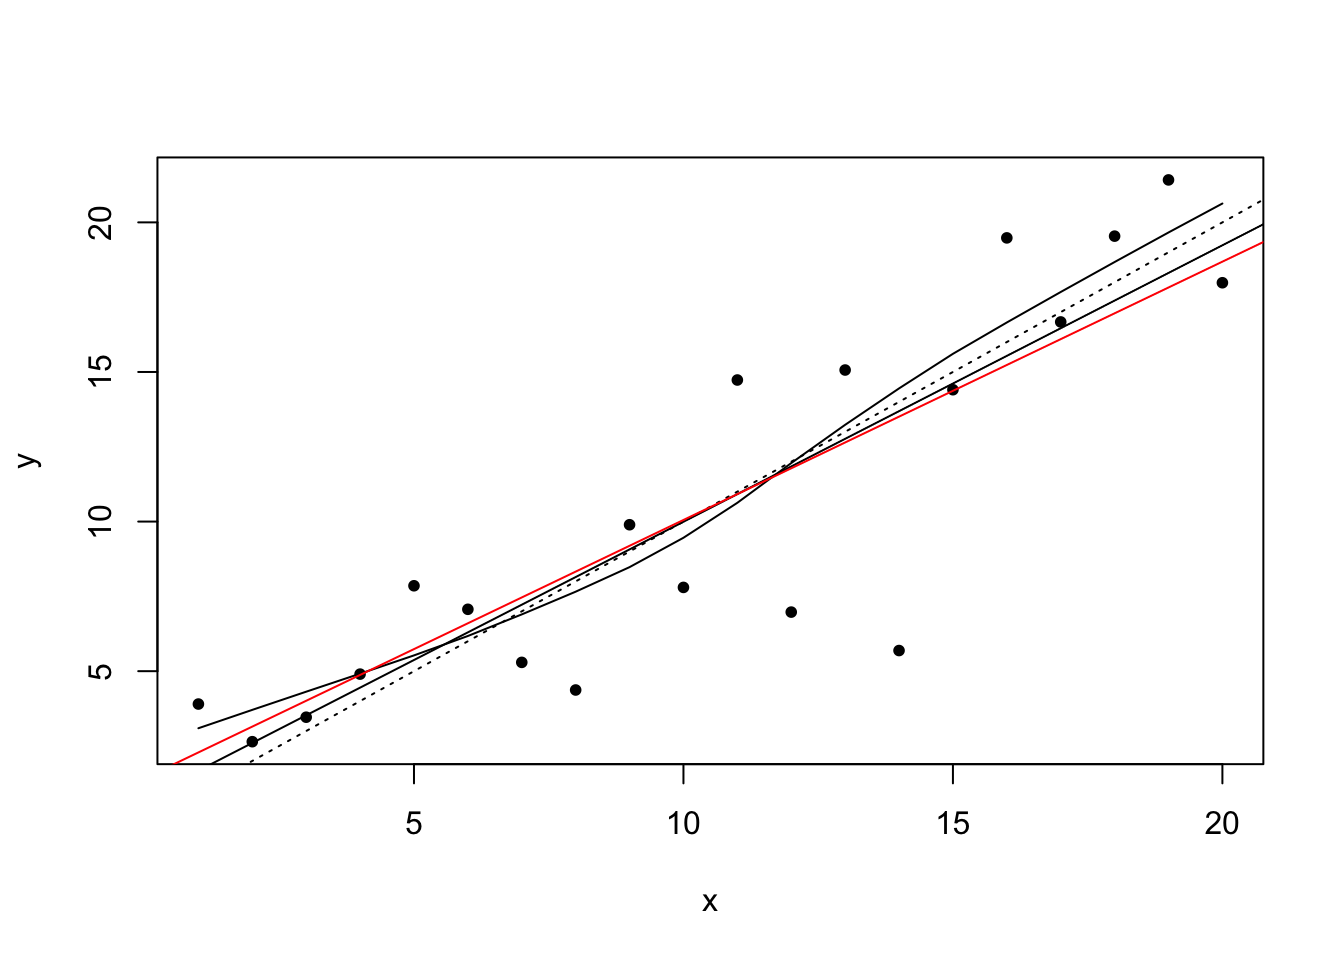
\includegraphics{DataProgramming_files/figure-latex/unnamed-chunk-6-1.pdf}

\begin{Shaded}
\begin{Highlighting}[]
\CommentTok{# A standard regression diagnostic plot to check for heteroscedasticity. Can you see it?}

\KeywordTok{plot}\NormalTok{(}\KeywordTok{fitted}\NormalTok{(fm), }\DataTypeTok{pch=}\DecValTok{20}\NormalTok{, }\KeywordTok{resid}\NormalTok{(fm), }\DataTypeTok{xlab=}\StringTok{"Fitted values"}\NormalTok{, }\DataTypeTok{ylab=}\StringTok{"Residuals"}\NormalTok{, }\DataTypeTok{main=}\StringTok{"Residuals vs Fitted"}\NormalTok{)}

\CommentTok{# How about now?}

\KeywordTok{abline}\NormalTok{(}\DecValTok{0}\NormalTok{,}\DecValTok{0}\NormalTok{, }\DataTypeTok{col=}\StringTok{"red"}\NormalTok{)  }
\end{Highlighting}
\end{Shaded}

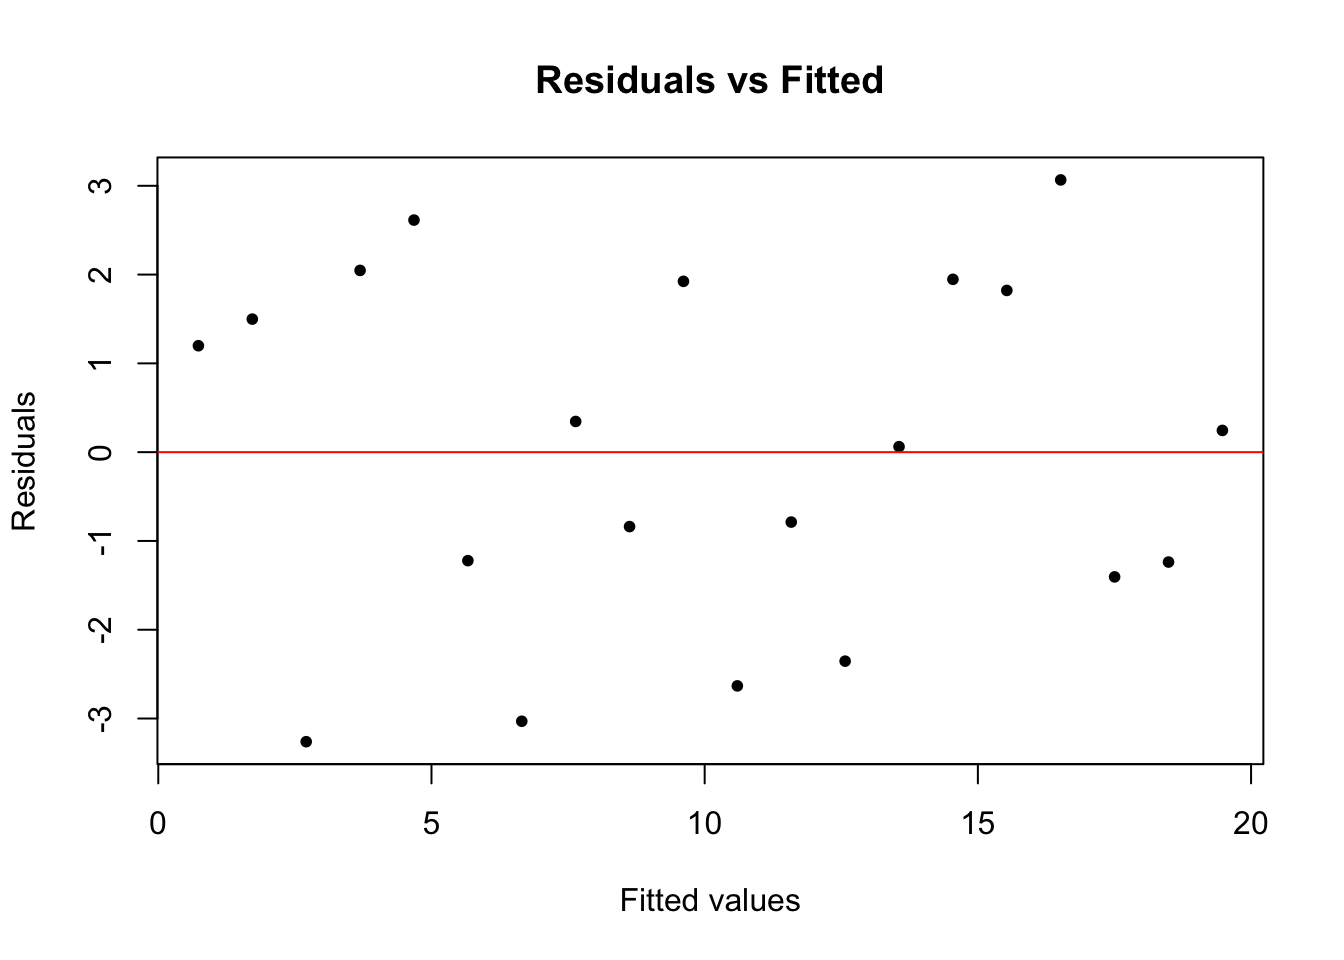
\includegraphics{DataProgramming_files/figure-latex/unnamed-chunk-6-2.pdf}

\begin{Shaded}
\begin{Highlighting}[]
\CommentTok{# A normal scores plot to check for skewness, kurtosis and outliers.}

\KeywordTok{qqnorm}\NormalTok{(}\KeywordTok{resid}\NormalTok{(fm), }\DataTypeTok{main=}\StringTok{"Residuals Rankit Plot"}\NormalTok{, }\DataTypeTok{pch=}\DecValTok{17}\NormalTok{)}
\end{Highlighting}
\end{Shaded}

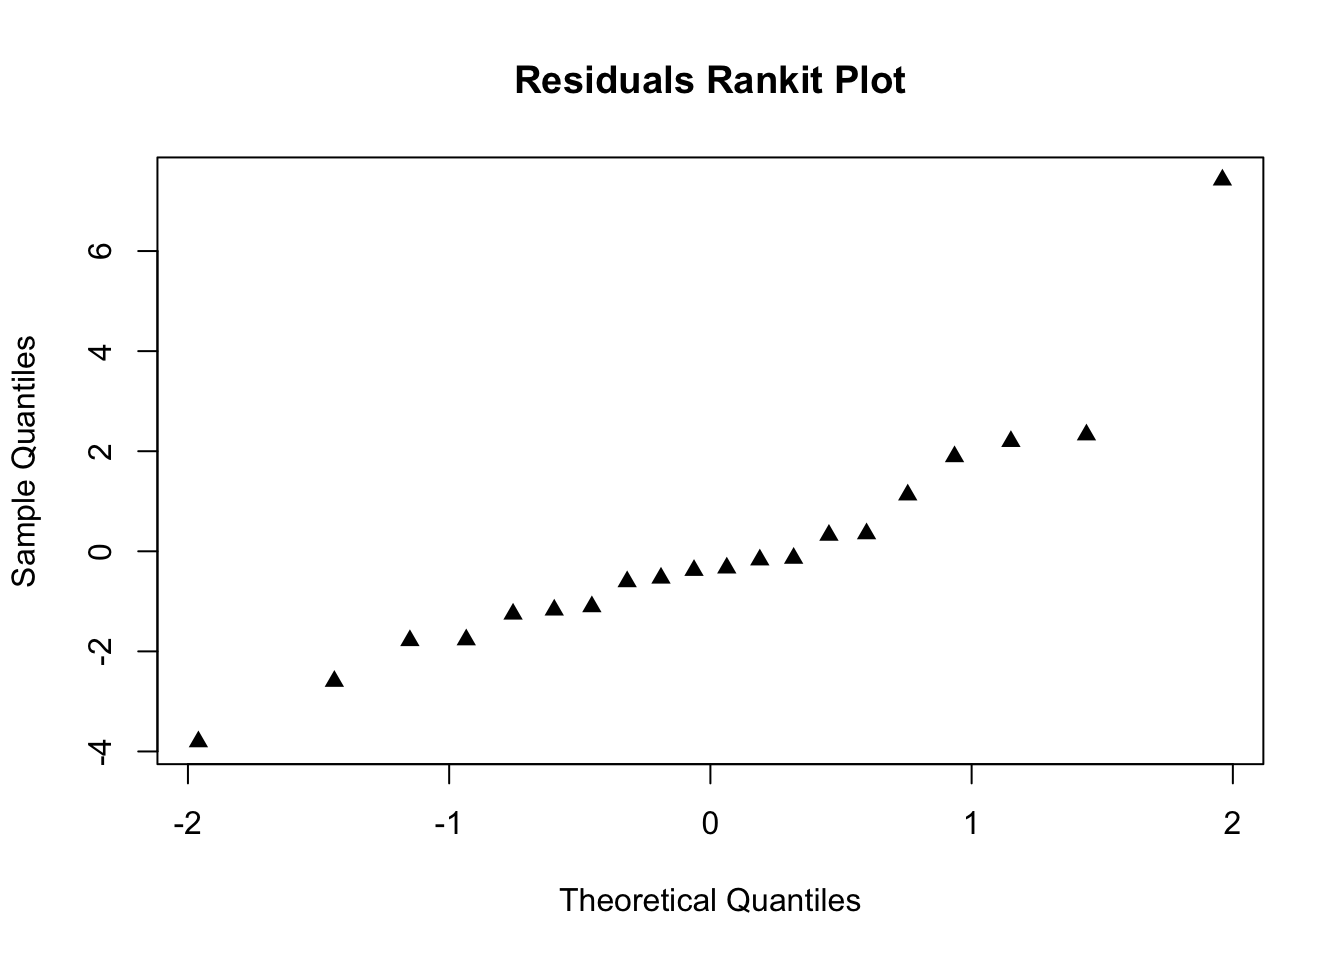
\includegraphics{DataProgramming_files/figure-latex/unnamed-chunk-6-3.pdf}

\begin{Shaded}
\begin{Highlighting}[]
\CommentTok{# Cleaning up}

\KeywordTok{rm}\NormalTok{(}\DataTypeTok{list =} \KeywordTok{ls}\NormalTok{())}
\end{Highlighting}
\end{Shaded}

\hypertarget{section-4}{%
\section{實例演示}\label{section-4}}

在本節中,我們將使用2016年台灣選舉與民主化研究計劃的數據作實例演示。台灣選舉和民主化研究(TEDS)是2001年開始的最長和最全面的選舉研究之一.TEDS通過不同的調查模式收集數據,包括面對面面談,電話採訪和網絡調查。有關TEDS的更多詳情,請訪問國立政治大學選舉研究中心網站 \url{https://esc.nccu.edu.tw/main.php}.

\emph{台灣選舉和民主化研究 2016}

\begin{Shaded}
\begin{Highlighting}[]
\CommentTok{# Import the TEDS 2016 data in Stata format using the haven package}
\CommentTok{## install.packages("haven")}

\KeywordTok{library}\NormalTok{(haven)}
\NormalTok{TEDS_}\DecValTok{2016}\NormalTok{ <-}\StringTok{ }\KeywordTok{read_stata}\NormalTok{(}\StringTok{"https://github.com/datageneration/home/blob/master/DataProgramming/data/TEDS_2016.dta?raw=true"}\NormalTok{)}

\CommentTok{# Prepare the analyze the Party ID variable }
\CommentTok{# Assign label to the values (1=KMT, 2=DPP, 3=NP, 4=PFP, 5=TSU, 6=NPP, 7="NA")}

\NormalTok{TEDS_}\DecValTok{2016}\OperatorTok{$}\NormalTok{PartyID <-}\StringTok{ }\KeywordTok{factor}\NormalTok{(TEDS_}\DecValTok{2016}\OperatorTok{$}\NormalTok{PartyID, }\DataTypeTok{labels=}\KeywordTok{c}\NormalTok{(}\StringTok{"KMT"}\NormalTok{,}\StringTok{"DPP"}\NormalTok{,}\StringTok{"NP"}\NormalTok{,}\StringTok{"PFP"}\NormalTok{, }\StringTok{"TSU"}\NormalTok{, }\StringTok{"NPP"}\NormalTok{,}\StringTok{"NA"}\NormalTok{))}
\end{Highlighting}
\end{Shaded}

PartyID (政黨認同變數):

\begin{Shaded}
\begin{Highlighting}[]
\CommentTok{# Check the variable}
\KeywordTok{attach}\NormalTok{(TEDS_}\DecValTok{2016}\NormalTok{)}
\end{Highlighting}
\end{Shaded}

\begin{verbatim}
## The following objects are masked from TEDS_2016 (pos = 13):
## 
##     age, Age, Arear, Blue, Career, Career8, District, DPP,
##     Econ_worse, econworse5, edu, Edu, Ethnic, female,
##     Govt_dont_care, Govt_for_public, green, Green, highincome,
##     income, income_nm, Independence, Inequality, inequality5, KMT,
##     lowincome, Mainland_father, Minnan_father, nI2, No_Party,
##     noparty, north, npp, Party, PartyID, pfp, pubwelf5, Sex,
##     South, sq, Taiwanese, Tondu, Tondu3, Unification, voteblue,
##     voteblue_nm, votedpp_1, votekmt, votekmt_1, votekmt_nm,
##     votetsai, votetsai_all, votetsai_nm, whitecollar
\end{verbatim}

\begin{Shaded}
\begin{Highlighting}[]
\KeywordTok{head}\NormalTok{(PartyID)}
\end{Highlighting}
\end{Shaded}

\begin{verbatim}
## [1] NA  NA  KMT NA  NA  DPP
## Levels: KMT DPP NP PFP TSU NPP NA
\end{verbatim}

\begin{Shaded}
\begin{Highlighting}[]
\KeywordTok{tail}\NormalTok{(PartyID)}
\end{Highlighting}
\end{Shaded}

\begin{verbatim}
## [1] NA  NA  DPP NA  NA  NA 
## Levels: KMT DPP NP PFP TSU NPP NA
\end{verbatim}

頻率表:

\begin{Shaded}
\begin{Highlighting}[]
\CommentTok{# Run a frequency table of the Party ID variable using the descr package}
\CommentTok{## install.packages("descr")}
\KeywordTok{library}\NormalTok{(descr)}
\KeywordTok{freq}\NormalTok{(TEDS_}\DecValTok{2016}\OperatorTok{$}\NormalTok{PartyID)}
\end{Highlighting}
\end{Shaded}

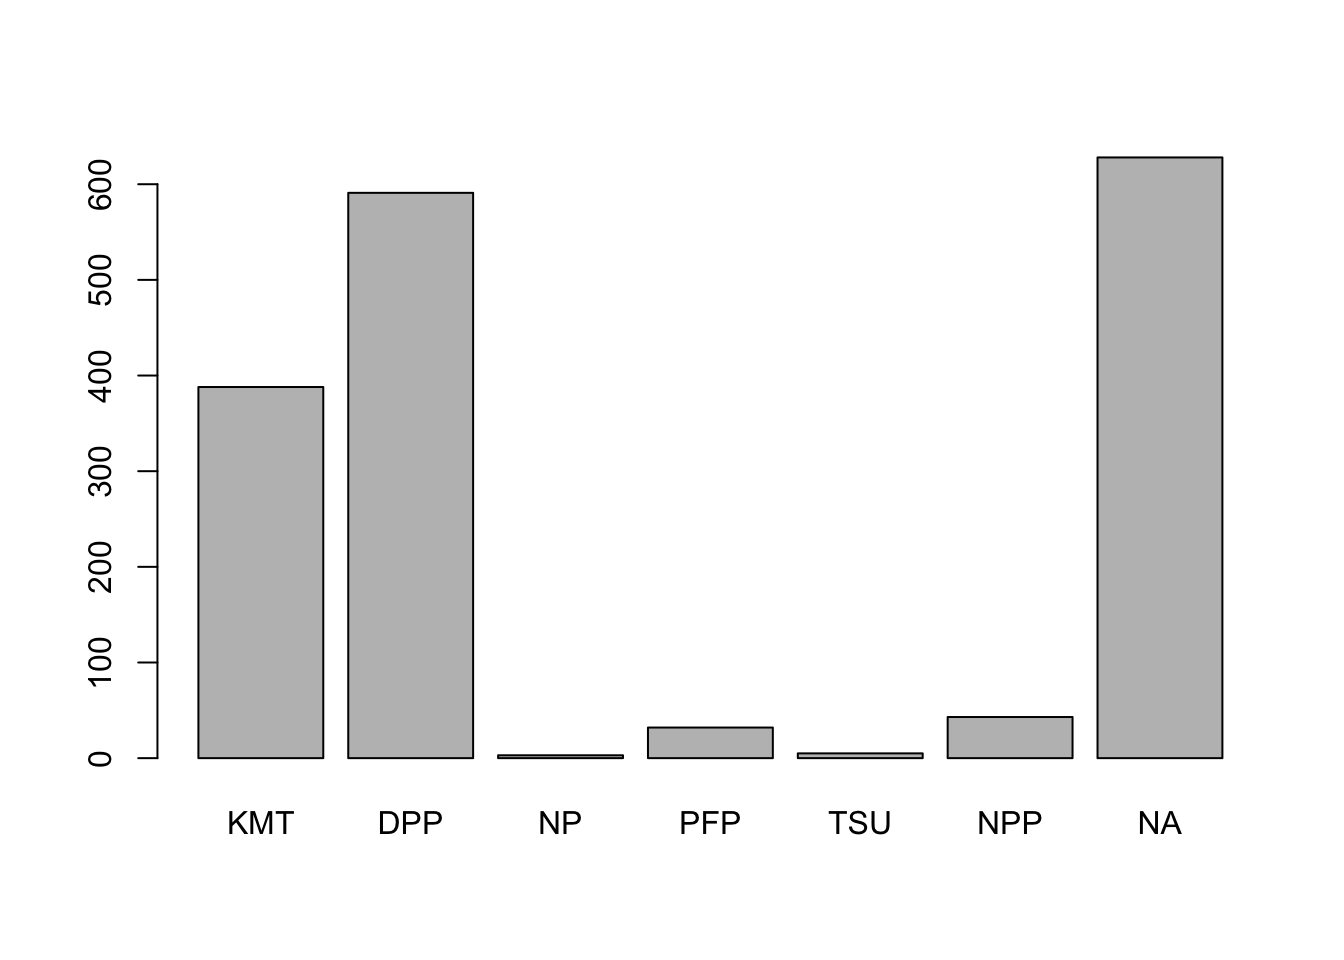
\includegraphics{DataProgramming_files/figure-latex/unnamed-chunk-9-1.pdf}

\begin{verbatim}
## TEDS_2016$PartyID 
##       Frequency  Percent
## KMT         388  22.9586
## DPP         591  34.9704
## NP            3   0.1775
## PFP          32   1.8935
## TSU           5   0.2959
## NPP          43   2.5444
## NA          628  37.1598
## Total      1690 100.0000
\end{verbatim}

圖表:

\begin{Shaded}
\begin{Highlighting}[]
\CommentTok{# Plot the Party ID variable}
\KeywordTok{ggplot}\NormalTok{(TEDS_}\DecValTok{2016}\NormalTok{, }\KeywordTok{aes}\NormalTok{(PartyID)) }\OperatorTok{+}\StringTok{ }
\StringTok{  }\KeywordTok{geom_bar}\NormalTok{()}
\end{Highlighting}
\end{Shaded}

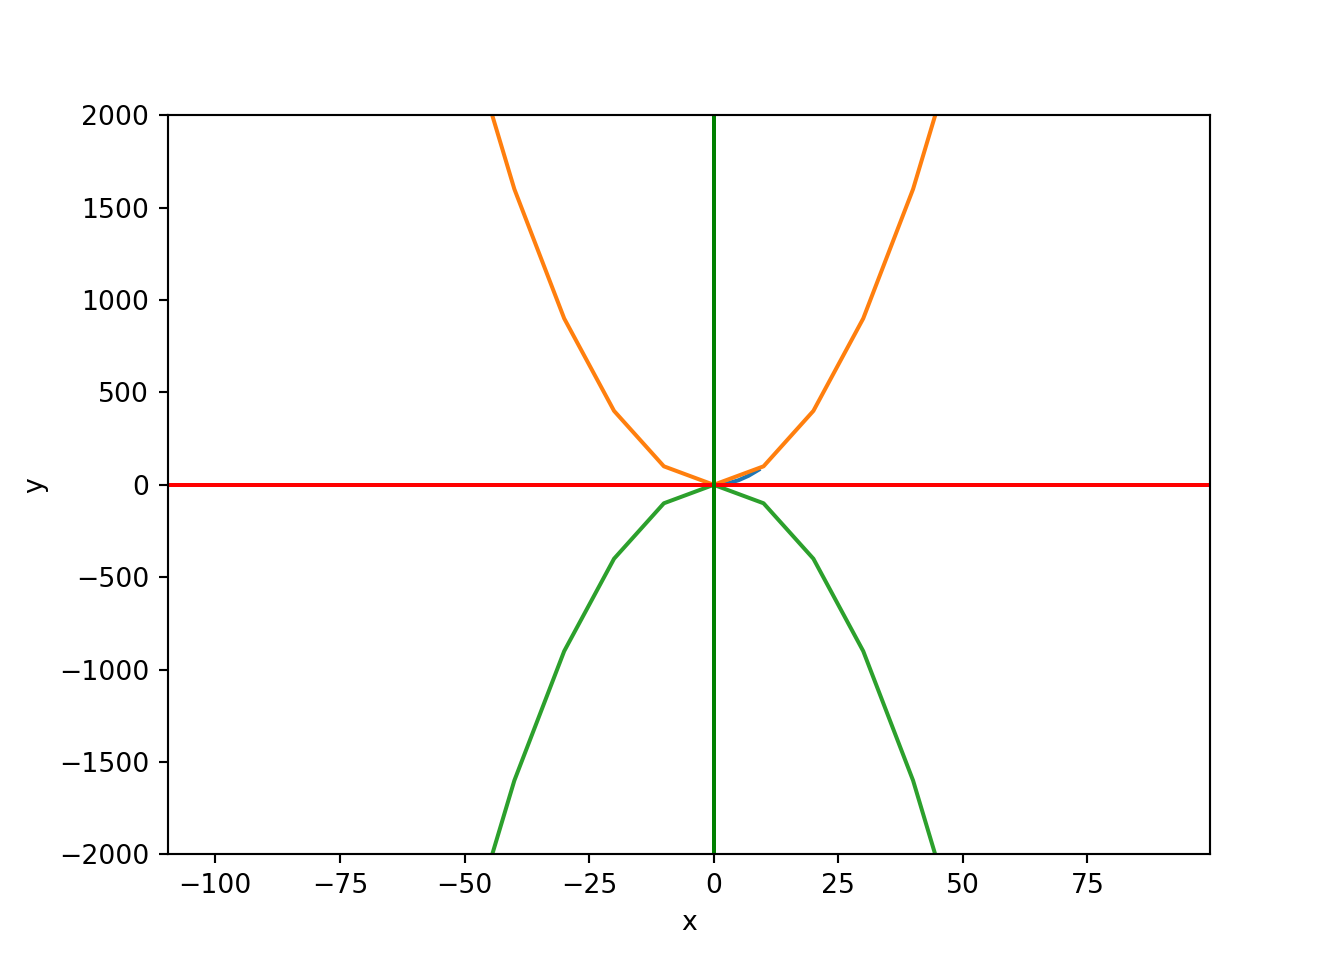
\includegraphics{DataProgramming_files/figure-latex/unnamed-chunk-10-1.pdf}

We can attend to more detail of the chart, such as adding labels to x and y axes, and calculating the percentage instead of counts.加入細節

\begin{Shaded}
\begin{Highlighting}[]
\KeywordTok{ggplot}\NormalTok{(TEDS_}\DecValTok{2016}\NormalTok{, }\KeywordTok{aes}\NormalTok{(PartyID)) }\OperatorTok{+}\StringTok{ }
\StringTok{  }\KeywordTok{geom_bar}\NormalTok{(}\KeywordTok{aes}\NormalTok{(}\DataTypeTok{y =}\NormalTok{ (..count..)}\OperatorTok{/}\KeywordTok{sum}\NormalTok{(..count..))) }\OperatorTok{+}\StringTok{ }
\StringTok{  }\KeywordTok{scale_y_continuous}\NormalTok{(}\DataTypeTok{labels=}\NormalTok{scales}\OperatorTok{::}\NormalTok{percent) }\OperatorTok{+}
\StringTok{  }\KeywordTok{ylab}\NormalTok{(}\StringTok{"Party Support (%)"}\NormalTok{) }\OperatorTok{+}\StringTok{ }
\StringTok{  }\KeywordTok{xlab}\NormalTok{(}\StringTok{"Taiwan Political Parties"}\NormalTok{)}
\end{Highlighting}
\end{Shaded}

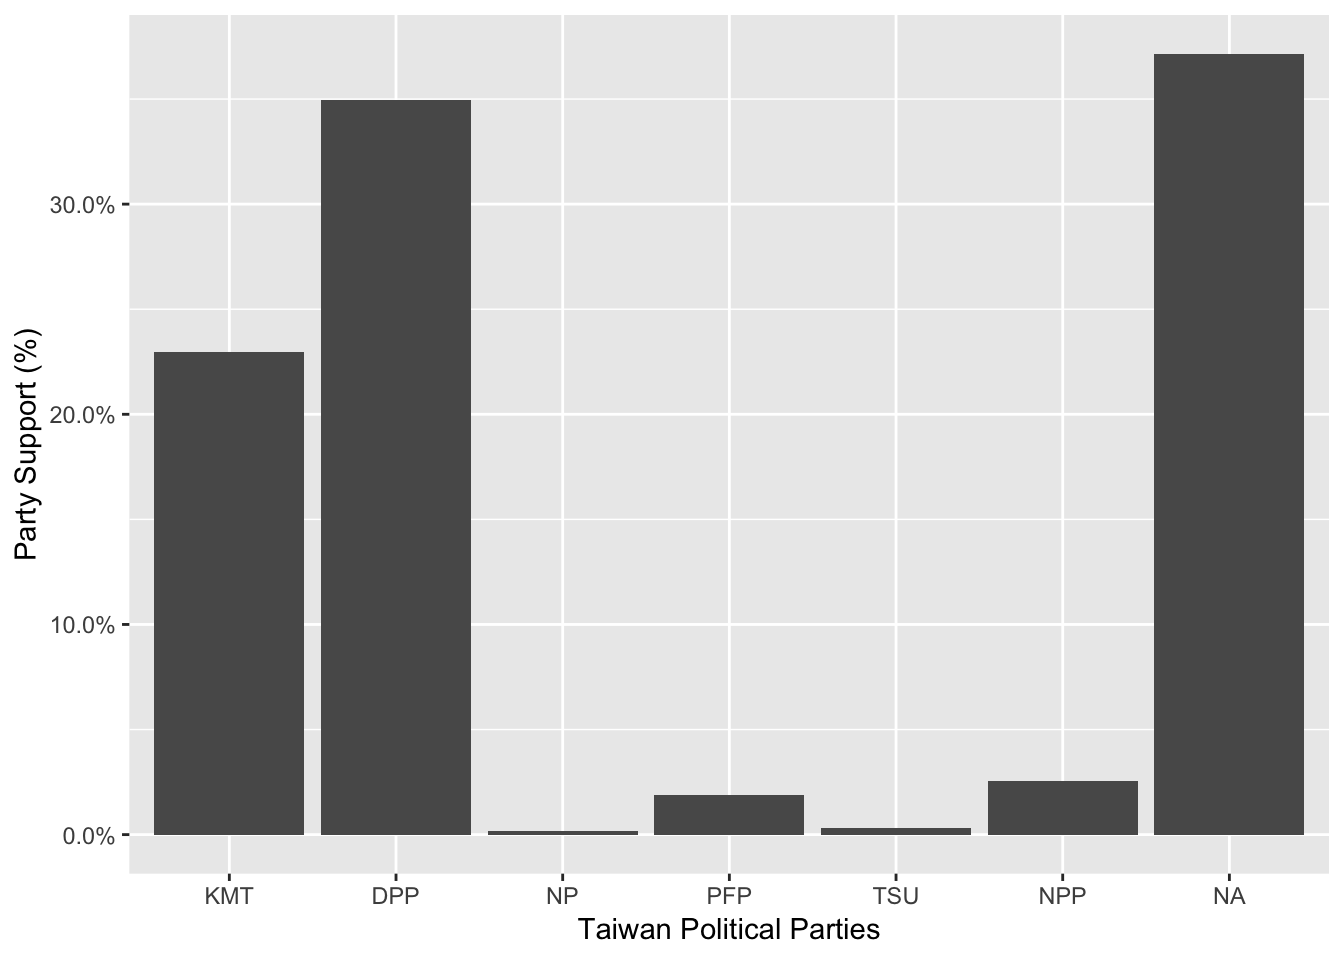
\includegraphics{DataProgramming_files/figure-latex/unnamed-chunk-11-1.pdf}

Adding colors, with another theme 加入顏色,設計:

\begin{Shaded}
\begin{Highlighting}[]
\KeywordTok{ggplot}\NormalTok{(TEDS_}\DecValTok{2016}\NormalTok{, }\KeywordTok{aes}\NormalTok{(PartyID)) }\OperatorTok{+}\StringTok{ }
\StringTok{  }\KeywordTok{geom_bar}\NormalTok{(}\KeywordTok{aes}\NormalTok{(}\DataTypeTok{y =}\NormalTok{ (..count..)}\OperatorTok{/}\KeywordTok{sum}\NormalTok{(..count..),}\DataTypeTok{fill=}\NormalTok{PartyID)) }\OperatorTok{+}\StringTok{ }
\StringTok{  }\KeywordTok{scale_y_continuous}\NormalTok{(}\DataTypeTok{labels=}\NormalTok{scales}\OperatorTok{::}\NormalTok{percent) }\OperatorTok{+}
\StringTok{  }\KeywordTok{ylab}\NormalTok{(}\StringTok{"Party Support (%)"}\NormalTok{) }\OperatorTok{+}\StringTok{ }
\StringTok{  }\KeywordTok{xlab}\NormalTok{(}\StringTok{"Taiwan Political Parties"}\NormalTok{) }\OperatorTok{+}
\StringTok{  }\KeywordTok{theme_bw}\NormalTok{()}
\end{Highlighting}
\end{Shaded}

\includegraphics{DataProgramming_files/figure-latex/unnamed-chunk-12-1.pdf}

Hold on, colors are not right!顏色有對嗎?

\begin{Shaded}
\begin{Highlighting}[]
\KeywordTok{ggplot}\NormalTok{(TEDS_}\DecValTok{2016}\NormalTok{, }\KeywordTok{aes}\NormalTok{(PartyID)) }\OperatorTok{+}\StringTok{ }
\StringTok{  }\KeywordTok{geom_bar}\NormalTok{(}\KeywordTok{aes}\NormalTok{(}\DataTypeTok{y =}\NormalTok{ (..count..)}\OperatorTok{/}\KeywordTok{sum}\NormalTok{(..count..),}\DataTypeTok{fill=}\NormalTok{PartyID)) }\OperatorTok{+}\StringTok{ }
\StringTok{  }\KeywordTok{scale_y_continuous}\NormalTok{(}\DataTypeTok{labels=}\NormalTok{scales}\OperatorTok{::}\NormalTok{percent) }\OperatorTok{+}
\StringTok{  }\KeywordTok{ylab}\NormalTok{(}\StringTok{"Party Support (%)"}\NormalTok{) }\OperatorTok{+}\StringTok{ }
\StringTok{  }\KeywordTok{xlab}\NormalTok{(}\StringTok{"Taiwan Political Parties"}\NormalTok{) }\OperatorTok{+}
\StringTok{  }\KeywordTok{theme_bw}\NormalTok{() }\OperatorTok{+}
\StringTok{  }\KeywordTok{scale_fill_manual}\NormalTok{(}\DataTypeTok{values=}\KeywordTok{c}\NormalTok{(}\StringTok{"steel blue"}\NormalTok{,}\StringTok{"forestgreen"}\NormalTok{,}\StringTok{"khaki1"}\NormalTok{,}\StringTok{"orange"}\NormalTok{,}\StringTok{"goldenrod"}\NormalTok{,}\StringTok{"yellow"}\NormalTok{,}\StringTok{"grey"}\NormalTok{))}
\end{Highlighting}
\end{Shaded}

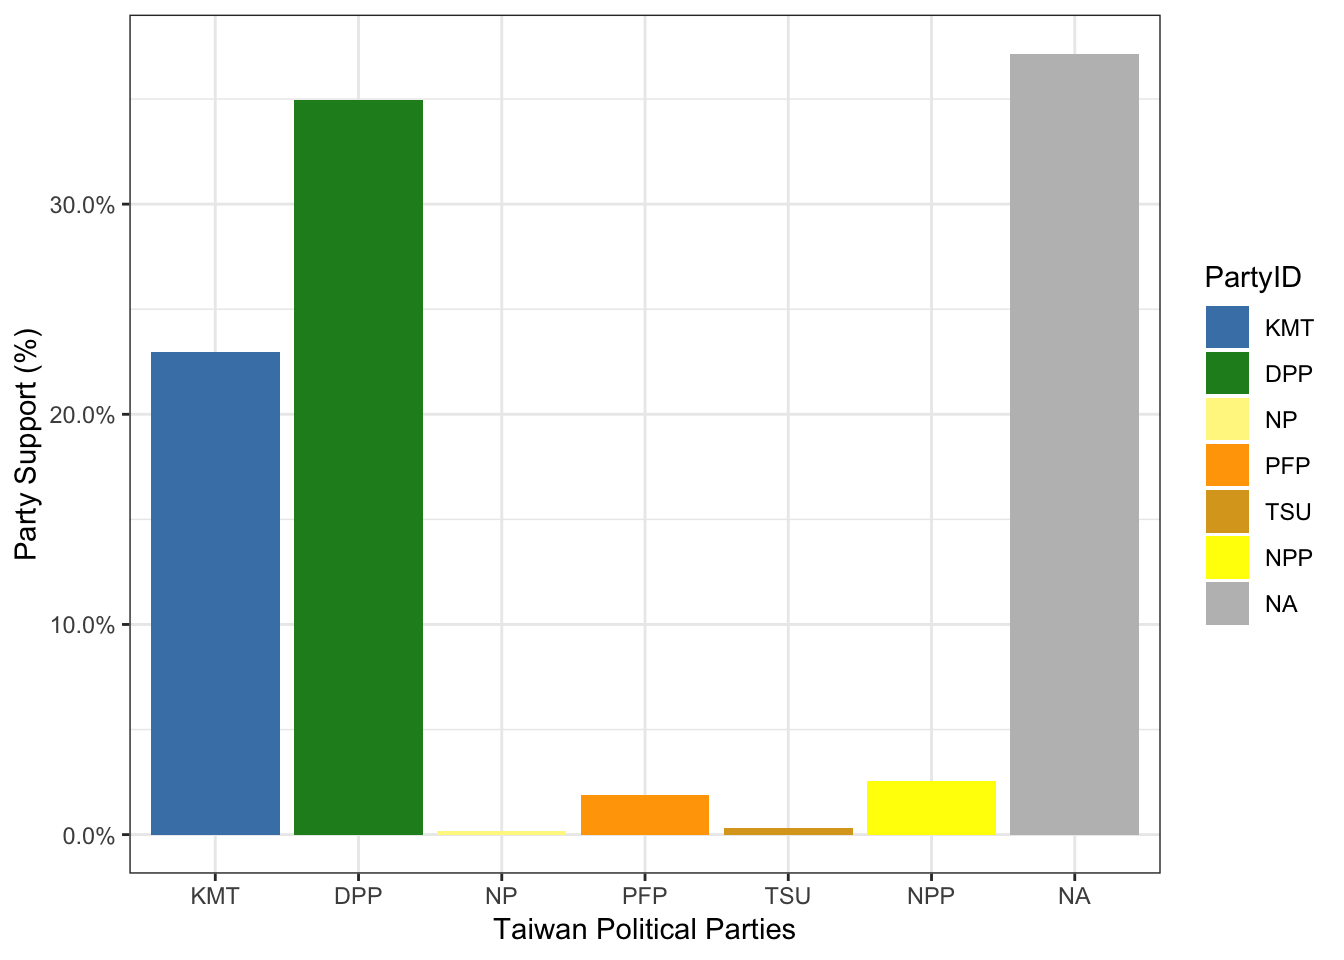
\includegraphics{DataProgramming_files/figure-latex/unnamed-chunk-13-1.pdf}

To make the chart more meaningful, we can use a package called tidyverse to manage the data. 更專業的圖表需要用tidyverse程式包

\begin{Shaded}
\begin{Highlighting}[]
\CommentTok{##install.packages("tidyverse")}
\KeywordTok{library}\NormalTok{(tidyverse)}
\NormalTok{TEDS_}\DecValTok{2016} \OperatorTok\StringTok{ }
\StringTok{  }\KeywordTok{count}\NormalTok{(PartyID) }\OperatorTok\StringTok{ }
\StringTok{  }\KeywordTok{mutate}\NormalTok{(}\DataTypeTok{perc =}\NormalTok{ n }\OperatorTok{/}\StringTok{ }\KeywordTok{nrow}\NormalTok{(TEDS_}\DecValTok{2016}\NormalTok{)) ->}\StringTok{ }\NormalTok{T2}
\KeywordTok{ggplot}\NormalTok{(T2, }\KeywordTok{aes}\NormalTok{(}\DataTypeTok{x =} \KeywordTok{reorder}\NormalTok{(PartyID, }\OperatorTok{-}\NormalTok{perc),}\DataTypeTok{y =}\NormalTok{ perc,}\DataTypeTok{fill=}\NormalTok{PartyID)) }\OperatorTok{+}\StringTok{ }
\StringTok{  }\KeywordTok{geom_bar}\NormalTok{(}\DataTypeTok{stat =} \StringTok{"identity"}\NormalTok{) }\OperatorTok{+}
\StringTok{  }\KeywordTok{ylab}\NormalTok{(}\StringTok{"Party Support (%)"}\NormalTok{) }\OperatorTok{+}\StringTok{ }
\StringTok{  }\KeywordTok{xlab}\NormalTok{(}\StringTok{"Taiwan Political Parties"}\NormalTok{) }\OperatorTok{+}
\StringTok{  }\KeywordTok{theme_bw}\NormalTok{() }\OperatorTok{+}
\StringTok{  }\KeywordTok{scale_fill_manual}\NormalTok{(}\DataTypeTok{values=}\KeywordTok{c}\NormalTok{(}\StringTok{"steel blue"}\NormalTok{,}\StringTok{"forestgreen"}\NormalTok{,}\StringTok{"khaki1"}\NormalTok{,}\StringTok{"orange"}\NormalTok{,}\StringTok{"goldenrod"}\NormalTok{,}\StringTok{"yellow"}\NormalTok{,}\StringTok{"grey"}\NormalTok{))}
\end{Highlighting}
\end{Shaded}

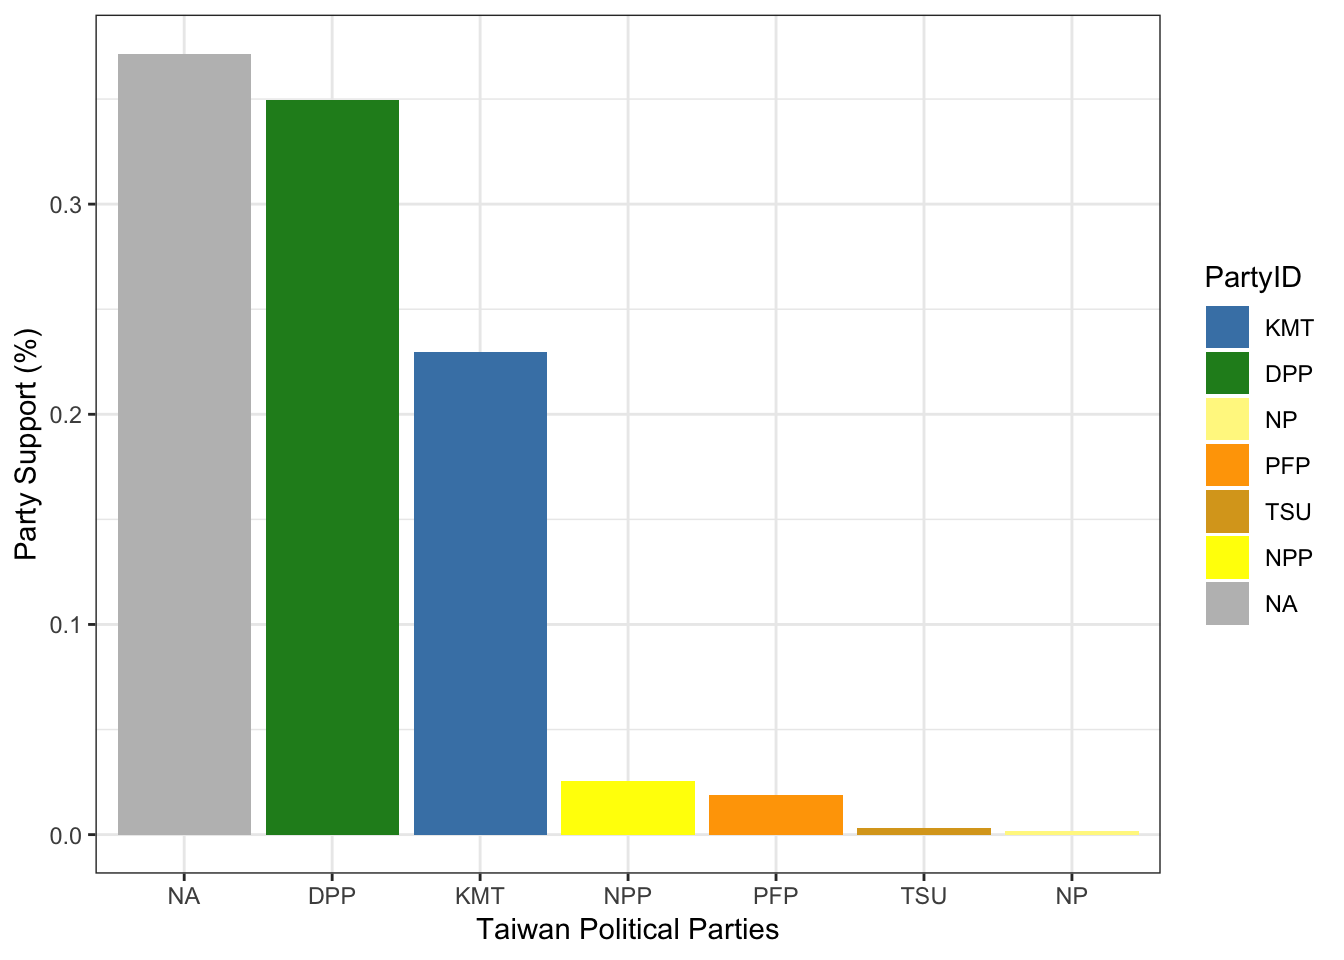
\includegraphics{DataProgramming_files/figure-latex/unnamed-chunk-14-1.pdf}

\hypertarget{section-5}{%
\section{作業}\label{section-5}}

利用以上的範例程式分析統獨(Tondu)變數

Analyze the Tondu (統獨)variable using the following procedures:

\begin{enumerate}
\def\labelenumi{\arabic{enumi}.}
\tightlist
\item
  Assign label to each category
\item
  Run a frequency table using descr
\item
  Plot the variable using ggplot2
\end{enumerate}

Hint:提示:

\begin{itemize}
\tightlist
\item
  Prepare the analyze the Tondu variable using these labels: (``Unification now'',``Status quo, unif. in future'',``Status quo, decide later'',``Status quo forever'', ``Status quo, indep. in future'', ``Independence now'',``No response'')
\item
  Sample codes:
\end{itemize}

\begin{verbatim}
TEDS_2016$Tondu<-factor(TEDS_2016$Tondu,labels=c("Unification now","Status quo, unif. in >future","Status quo, decide later","Status quo forever", >"Status quo, indep. in future", "Independence now","No >response"))
\end{verbatim}

\hypertarget{r-4}{%
\section{R資源推薦:}\label{r-4}}

\begin{itemize}
\tightlist
\item
  \href{http://journal.r-project.org/}{The R Journal}
\item
  \href{http://cran.r-project.org/doc/manuals/R-intro.pdf}{Introduction to R by W. N. Venables, D. M. Smith and the R Core Team}
\item
  \href{http://www.ats.ucla.edu/stat/r/seminars/intro.htm}{Introduction to R Seminar at UCLA}
\item
  \href{https://dss.princeton.edu/training/}{Getting Started in Data Analysis using Stata and R by Data and Statistical Services, Princeton University}
\end{itemize}

\hypertarget{python}{%
\chapter{Python程式設計}\label{python}}

\hypertarget{python-1}{%
\section{什麼是Python?}\label{python-1}}

\begin{itemize}
\tightlist
\item
  直譯式,高階計算機語言
\item
  由荷蘭程式設計師Guido van Rossum發明
\item
  以電視節目\emph{Monty Python's Flying Circus} (飛行馬戲團)中的Monty Python 命名
\item
  開源程式語言
\end{itemize}

\begin{figure}

\hfill{}
\includegraphics[width=0.5\linewidth]{Pythoninventor} 

\caption{Python Inventor Guido van Rossum}\label{fig:Pythoninventor}
\end{figure}

\hypertarget{python-2}{%
\subsection{為何選擇Python?}\label{python-2}}

\begin{itemize}
\tightlist
\item
  簡單
\item
  科學計算和數據科學特定領域具有大型生態系統
\item
  用戶們建構的套件
\item
  數據管理

  \begin{itemize}
  \tightlist
  \item
    互聯網數據
  \item
    大數據處理
  \end{itemize}
\end{itemize}

\hypertarget{python-3}{%
\section{Python基本程式包:}\label{python-3}}

\begin{enumerate}
\def\labelenumi{\arabic{enumi}.}
\tightlist
\item
  NumPy - 操縱基於同構數組的數據
\item
  Pandas - 操縱建構和標記數據
\item
  SciPy - 用於常見的科學計算任務
\item
  Matplotlib - 數據視覺化
\item
  IPython - 使用Jupyter筆記本交互式執行和共享程式碼
\item
  Scikit-Learn - 機器學習
\end{enumerate}

\hypertarget{python-ide}{%
\section{Python IDE整合式開發環境}\label{python-ide}}

整合式開發環境的選擇至關重要!有很多IDE可用於python編程和開發。僅舉幾例:

\begin{itemize}
\tightlist
\item
  IDLE
\item
  Pycharm
\item
  Jupyter Notebook
\item
  Spyder
\item
  Rodeo
\item
  R Studio
\end{itemize}

\hypertarget{section-6}{%
\section{基本操作和賦值}\label{section-6}}

\begin{Shaded}
\begin{Highlighting}[]
\CommentTok{# Python example program 0}
\CommentTok{# Some basics}

\CommentTok{# Print a one-line message}
\BuiltInTok{print}\NormalTok{ (}\StringTok{"Hello NCHU 中興大學 friends!!"}\NormalTok{)}

\CommentTok{# Create some variables}
\end{Highlighting}
\end{Shaded}

\begin{verbatim}
## Hello NCHU 中興大學 friends!!
\end{verbatim}

\begin{Shaded}
\begin{Highlighting}[]
\NormalTok{x}\OperatorTok{=}\DecValTok{5}
\NormalTok{y}\OperatorTok{=}\DecValTok{3}

\CommentTok{# Perform some mathematical operations}
\NormalTok{x}\OperatorTok{*}\NormalTok{y}
\end{Highlighting}
\end{Shaded}

\begin{verbatim}
## 15
\end{verbatim}

\begin{Shaded}
\begin{Highlighting}[]
\NormalTok{x}\OperatorTok{**}\NormalTok{y}
\end{Highlighting}
\end{Shaded}

\begin{verbatim}
## 125
\end{verbatim}

\begin{Shaded}
\begin{Highlighting}[]
\NormalTok{x}\OperatorTok{%}\NormalTok{y}
\end{Highlighting}
\end{Shaded}

\begin{verbatim}
## 2
\end{verbatim}

\hypertarget{section-7}{%
\subsection{導入套件庫}\label{section-7}}

\begin{Shaded}
\begin{Highlighting}[]
\CommentTok{#Import Python Libraries}
\ImportTok{import}\NormalTok{ numpy }\ImportTok{as}\NormalTok{ np}
\ImportTok{import}\NormalTok{ scipy }\ImportTok{as}\NormalTok{ sp}
\ImportTok{import}\NormalTok{ pandas }\ImportTok{as}\NormalTok{ pd}
\ImportTok{import}\NormalTok{ matplotlib }\ImportTok{as}\NormalTok{ mpl}
\ImportTok{import}\NormalTok{ seaborn }\ImportTok{as}\NormalTok{ sns}
\ImportTok{import}\NormalTok{ pandas }\ImportTok{as}\NormalTok{ pd}
\ImportTok{import}\NormalTok{ matplotlib.pyplot }\ImportTok{as}\NormalTok{ plt}
\ImportTok{import}\NormalTok{ seaborn }\ImportTok{as}\NormalTok{ sns}
\end{Highlighting}
\end{Shaded}

\hypertarget{section-8}{%
\subsection{載入資料}\label{section-8}}

\begin{Shaded}
\begin{Highlighting}[]

\CommentTok{# Import a text file in csv format}
\ImportTok{import}\NormalTok{ pandas }\ImportTok{as}\NormalTok{ pd}
\NormalTok{CO2 }\OperatorTok{=}\NormalTok{ pd.read_csv(}\StringTok{"https://raw.githubusercontent.com/kho777/data-visualization/master/data/CO2.csv"}\NormalTok{)}

\CommentTok{# Take a glimpse of the data file}
\NormalTok{CO2.head()}
\end{Highlighting}
\end{Shaded}

\begin{verbatim}
##                country               CO2 _kt  CO2pc  CO2percent
## 0                       Australia    446,348   18.6       1.23%
## 1                   United States  5,172,336   16.1      14.26%
## 2                    Saudi Arabia    505,565   16.0       1.39%
## 3                          Canada    555,401   15.5       1.53%
## 4                          Russia  1,760,895   12.3       4.86%
\end{verbatim}

\hypertarget{section-9}{%
\subsection{簡單的繪圖}\label{section-9}}

\begin{Shaded}
\begin{Highlighting}[]
\CommentTok{# Creating variables}
\NormalTok{xs }\OperatorTok{=}\NormalTok{ [}\DecValTok{1}\NormalTok{,}\DecValTok{3}\NormalTok{,}\DecValTok{5}\NormalTok{,}\DecValTok{7}\NormalTok{,}\DecValTok{9}\NormalTok{]}
\NormalTok{ys }\OperatorTok{=}\NormalTok{ [x}\OperatorTok{**}\DecValTok{2} \ControlFlowTok{for}\NormalTok{ x }\KeywordTok{in}\NormalTok{ xs]}

\CommentTok{# Simple plot}
\NormalTok{plt.plot(xs, ys)}

\NormalTok{xs }\OperatorTok{=} \BuiltInTok{range}\NormalTok{(}\OperatorTok{-}\DecValTok{100}\NormalTok{,}\DecValTok{100}\NormalTok{,}\DecValTok{10}\NormalTok{)}
\NormalTok{x2 }\OperatorTok{=}\NormalTok{ [x}\OperatorTok{**}\DecValTok{2} \ControlFlowTok{for}\NormalTok{ x }\KeywordTok{in}\NormalTok{ xs]}
\NormalTok{negx2 }\OperatorTok{=}\NormalTok{ [}\OperatorTok{-}\NormalTok{x}\OperatorTok{**}\DecValTok{2} \ControlFlowTok{for}\NormalTok{ x }\KeywordTok{in}\NormalTok{ xs]}

\CommentTok{# Combined plot}

\NormalTok{plt.plot(xs, x2)}
\NormalTok{plt.plot(xs, negx2)}
\NormalTok{plt.xlabel(}\StringTok{"x"}\NormalTok{)}
\NormalTok{plt.ylabel(}\StringTok{"y"}\NormalTok{)}
\NormalTok{plt.ylim(}\OperatorTok{-}\DecValTok{2000}\NormalTok{, }\DecValTok{2000}\NormalTok{)}
\end{Highlighting}
\end{Shaded}

\begin{verbatim}
## (-2000, 2000)
\end{verbatim}

\begin{Shaded}
\begin{Highlighting}[]
\NormalTok{plt.axhline(}\DecValTok{0}\NormalTok{,color}\OperatorTok{=}\StringTok{"red"}\NormalTok{) }\CommentTok{# horiz line}
\NormalTok{plt.axvline(}\DecValTok{0}\NormalTok{,color}\OperatorTok{=}\StringTok{"green"}\NormalTok{) }\CommentTok{# vert line}
\NormalTok{plt.show()}
\end{Highlighting}
\end{Shaded}

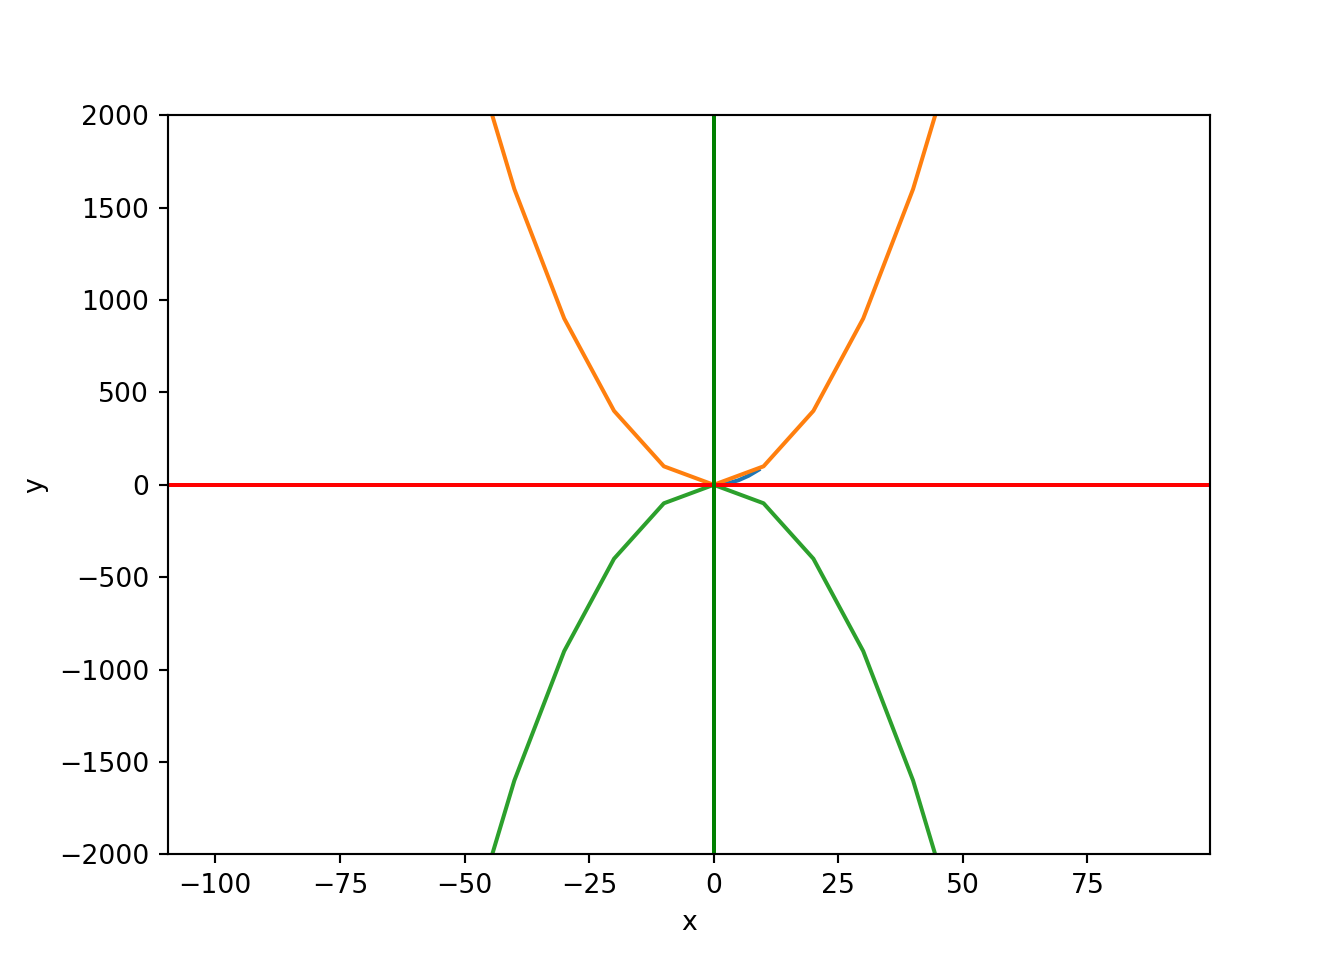
\includegraphics{DataProgramming_files/figure-latex/unnamed-chunk-18-1.pdf}

\hypertarget{section-10}{%
\subsection{資料視覺化}\label{section-10}}

\begin{Shaded}
\begin{Highlighting}[]

\ImportTok{import}\NormalTok{ matplotlib.pyplot }\ImportTok{as}\NormalTok{ plt}

\NormalTok{x }\OperatorTok{=}\NormalTok{ np.linspace(}\DecValTok{0}\NormalTok{, }\DecValTok{2}\NormalTok{, }\DecValTok{100}\NormalTok{)}
\NormalTok{plt.plot(x, x, label}\OperatorTok{=}\StringTok{'linear'}\NormalTok{,color}\OperatorTok{=}\StringTok{"pink"}\NormalTok{)}
\NormalTok{plt.plot(x, x}\OperatorTok{**}\DecValTok{2}\NormalTok{, label}\OperatorTok{=}\StringTok{'quadratic'}\NormalTok{)}
\NormalTok{plt.plot(x, x}\OperatorTok{**}\DecValTok{3}\NormalTok{, label}\OperatorTok{=}\StringTok{'cubic'}\NormalTok{)}
\NormalTok{plt.xlabel(}\StringTok{'x'}\NormalTok{,fontsize}\OperatorTok{=}\DecValTok{12}\NormalTok{,fontweight}\OperatorTok{=}\StringTok{'bold'}\NormalTok{)}
\NormalTok{plt.ylabel(}\StringTok{'y'}\NormalTok{,fontsize}\OperatorTok{=}\DecValTok{12}\NormalTok{,fontweight}\OperatorTok{=}\StringTok{'bold'}\NormalTok{)}

\NormalTok{plt.title(}\StringTok{"Plotting functions: Linear, quadratic and cubic"}\NormalTok{, fontsize}\OperatorTok{=}\DecValTok{16}\NormalTok{,fontweight}\OperatorTok{=}\StringTok{'bold'}\NormalTok{)}
\end{Highlighting}
\end{Shaded}

\includegraphics{DataProgramming_files/figure-latex/unnamed-chunk-19-1.pdf}

\hypertarget{section-11}{%
\section{作業}\label{section-11}}

This exercise is designed to run in class. Students are advised to install Anaconda 3 to own computer.

\begin{enumerate}
\def\labelenumi{\arabic{enumi}.}
\tightlist
\item
  Launch Jupyter Notebook from Anaconda
\item
  On Applications pulldown menu, choose anaconda3
\item
  Run sample programs from class GitHub (\url{https://github.com/datageneration/dataprogramming/})
\end{enumerate}

\hypertarget{python-4}{%
\section{Python資源推薦:}\label{python-4}}

\begin{itemize}
\tightlist
\item
  \href{https://jakevdp.github.io/WhirlwindTourOfPython/00-introduction.html}{A Whirlwind Tool of Python}: Getting started
\item
  \href{https://datacamp.com}{Datacamp}: Online training courses
\item
  \href{http://matplotlib.org}{Matplotlib.org}: Data visualization
\end{itemize}

\hypertarget{javascript}{%
\chapter{JavaScript}\label{javascript}}

\hypertarget{javascript-1}{%
\section{什麼是JavaScript?}\label{javascript-1}}

\begin{figure}

\hfill{}\includegraphics[width=0.25\linewidth]{JavaScriptinventor} 

\caption{JavaScript Inventor Brendan Eich}\label{fig:JavaScriptinventor}
\end{figure}

\begin{itemize}
\tightlist
\item
  JavaScript與Java無關
\item
  由Brendan Eich於1995年創建
\item
  最初是作為Web瀏覽器(客戶端)的原型語言開發的。
\item
  現在也在伺服器端(Node.js)中使用。
\item
  與Java無關,只是為了營銷目的而命名。
\item
  C風格的語法,但從功能程式設計中獲得靈感
\item
  for,while,continue,break,if / else,switch類似於C.
\item
  運算符(+, - ,*,/,%)也類似(除了==,!=,\textbar\textbar)
\item
  包括map,reduce,forEach等函數操作。
\end{itemize}

\hypertarget{javascript-2}{%
\subsection{JavaScript數據類型}\label{javascript-2}}

數據類型

\begin{itemize}
\tightlist
\item
  數字:42,3.14159
\item
  邏輯值:真,假
\item
  字串:``你好'',``台灣''
\item
  空值
\item
  undefined * - undefined不為null(空值)!
\end{itemize}

\hypertarget{javascript-object-notation-json}{%
\subsection{JavaScript Object Notation (JSON)}\label{javascript-object-notation-json}}

\begin{itemize}
\tightlist
\item
  JavaScript Object Notation 對象表示法
\item
  JavaScript作為存儲資料的XML替代方案
\item
  範例:
\end{itemize}

{[}\{``Station'':``Alishan'',``Temperature'':14.5,``Precipitation'':812.4,``Humidity'':95,``Pressure'':762.5,``dayrain'':30\},\ldots.{]}

\hypertarget{d3}{%
\section{什麼是D3?}\label{d3}}

\begin{itemize}
\tightlist
\item
  D3代表數據驅動文檔。-d3.js(D3)是``用於根據數據操作文檔的JavaScript庫''。
\item
  D3可以與HTML和CSS(以及其他)結合使用,以視覺化網頁上的數據。
\item
  這是一個開放的框架。
\item
  它在程式腳本中嵌入或包含數據資料,以在網頁中創建圖像。
\end{itemize}

\begin{quote}
``With D3, designers selectively bind input data to arbitrary document elements, applying dynamic transforms to both generate and modify content.''
``使用D3,設計人員有選擇地將輸入數據綁定到任意文檔元素,應用動態轉換來生成和修改內容。``

---\href{https://data3.mprog.nl/course/15\%20Readings/60\%20Reading\%206/Bostock_D3.pdf}{Bostock, Ogievetsky and Heer, 2011}
\end{quote}

\hypertarget{d3web}{%
\subsection{D3和Web文檔}\label{d3web}}

\begin{itemize}
\tightlist
\item
  D3是基於Web的,使用以下組件:

  \begin{itemize}
  \tightlist
  \item
    HTML(超文本標記語言)
  \item
    CSS(串樣式列表)
  \item
    JavaScript(JS)
  \item
    SVG(可縮放向量圖形),解釋圖形輸出
    以上所有內容都可以使用文本編輯器進行編碼。輸出需要帶有JavaScript控制台的瀏覽器
  \end{itemize}
\end{itemize}

\hypertarget{sample-d3-graphics}{%
\subsection{Sample D3 graphics}\label{sample-d3-graphics}}

Interactive Ladder Graph 交互式梯形圖

\begin{figure}
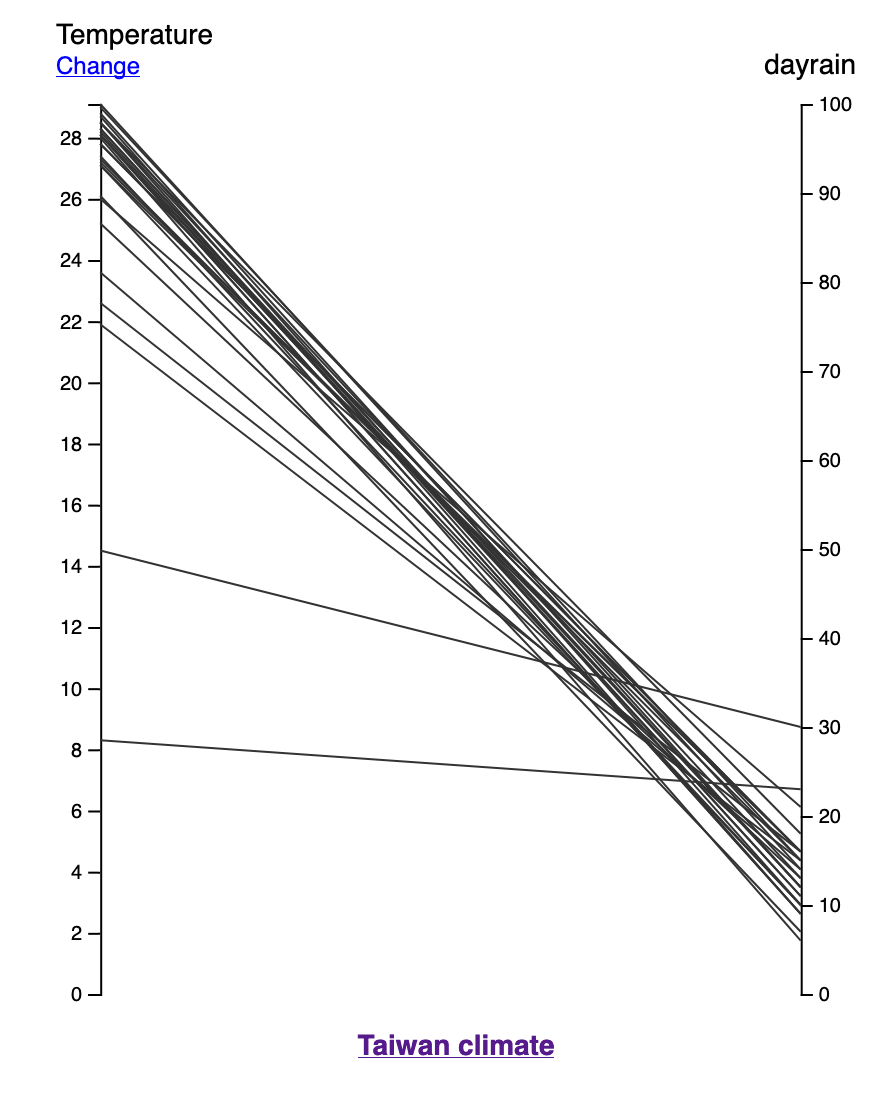
\includegraphics[width=0.5\linewidth]{laddergraph_twclimate} \caption{D3: Ladder graph}\label{fig:D3laddergraph}
\end{figure}

Click \href{https://karl-ho.github.io/D3/lg_twclimate/index.html}{here} to access the online version

Interactive Aster Graph

\begin{figure}
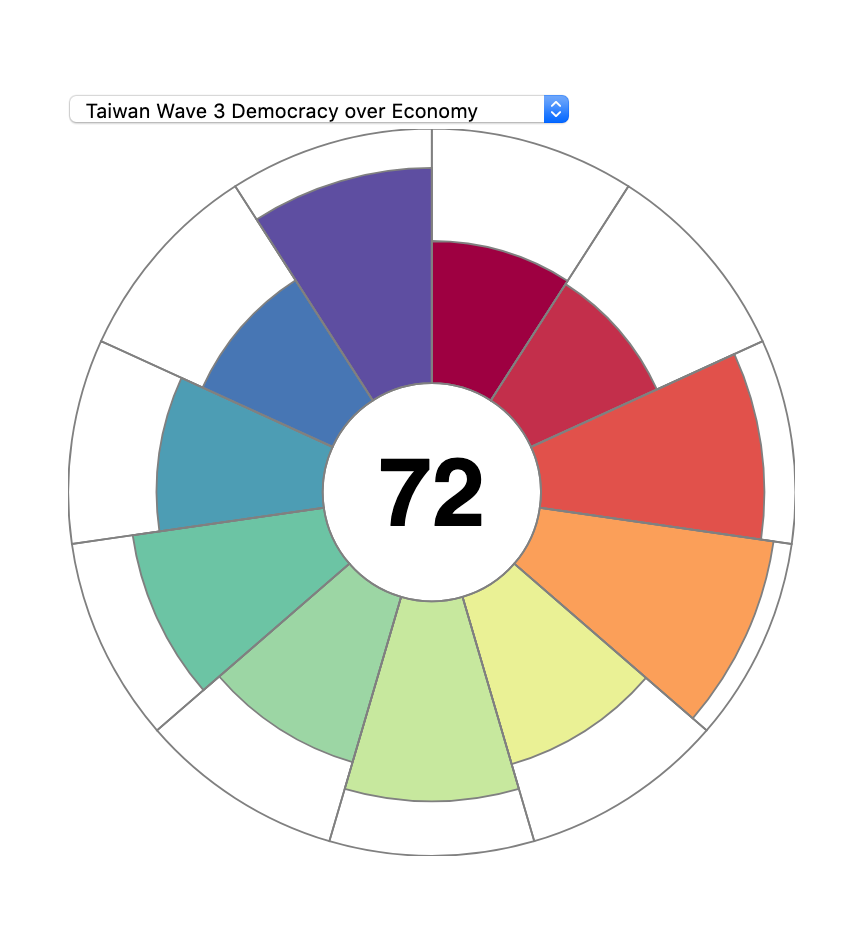
\includegraphics[width=0.5\linewidth]{astergraph_twhkdemocracy} \caption{D3: Aster graph}\label{fig:D3astergraph}
\end{figure}

Click \href{https://www.utdallas.edu/~kyho/present/aster/lpm.html}{here} to access the online version

\href{https://karl-ho.github.io/D3/createnetwork/index.html}{Interactive Network Graph}

\hypertarget{section-12}{%
\chapter{總結}\label{section-12}}

本文件為``資料程式設計''課程提供了簡要說明和示範程式,涵蓋了數據科學的基本程式設計。本卷中包含的語言主要是R,Python和JavaScript。將有更多的發展來添加材料和樣本程式,以將這些文件構建成一個完整的資料科學程式集。

更多資料及程式範例可從本課程GitHub獲取:

\url{https://www.github.com/datageneration/dataprogramming/}

\bibliography{book.bib,packages.bib}


\end{document}
